\documentclass[11pt]{article}

\usepackage{amsmath,amssymb,amsthm}
\usepackage{hyperref}
\usepackage{geometry}
\usepackage{booktabs}
\usepackage{tabularx}
\usepackage{ragged2e}
\usepackage{tcolorbox}
\usepackage{tikz}
\usetikzlibrary{positioning, arrows.meta, calc}
\usepackage{enumitem} 

\geometry{margin=1in}
\theoremstyle{plain}
\newtheorem{theorem}{Theorem}
\newtheorem{lemma}{Lemma}
\newtheorem{corollary}{Corollary}
\newtheorem{proposition}{Proposition}

\theoremstyle{definition}
\newtheorem{definition}{Definition}

\theoremstyle{remark}
\newtheorem{remark}{Remark}

\title{Second-Order Constraint Geometry}
\author{A. R. Wells \\ Dual-Frame Research Group}
\date{\today}

% --- Dirac notation (minimal, no extra package dependency) ---
\newcommand{\ket}[1]{\left|#1\right\rangle}
\newcommand{\bra}[1]{\left\langle#1\right|}
\newcommand{\braket}[2]{\left\langle#1\,\middle|\,#2\right\rangle}
\newcommand{\ketbra}[2]{\left|#1\right\rangle\!\left\langle#2\right|}

% (Optional helpers if you use them elsewhere)
\newcommand{\Tr}{\operatorname{Tr}}
\newcommand{\I}{\mathbb{I}}

\begin{document}
\maketitle

% --- Front matter ---
\begin{abstract}
Many physical and computational systems exhibit behavior that depends not only on
their instantaneous state, but on the ordering, admissibility, or history of prior
transformations. Standard state-based formalisms accommodate such behavior only by augmenting the state with hidden registers, contextual labels, or implicit memory.
This effectively blurs the distinction between genuine physical structure and bookkeeping artifacts.

In this work we introduce \emph{second-order constraint geometry} ($\Sigma_2$), a
geometric framework defined over admissible trajectories rather than instantaneous
states. $\Sigma_2$ formalizes when and why state descriptions are insufficient, without
appeal to hidden variables or enlarged state spaces. The framework characterizes
order-sensitive and history-dependent phenomena as arising from constraints on
admissible sequences of transformations, rather than from additional state content.

We show that $\Sigma_2$ provides a principled criterion distinguishing legitimate
state evolution from illegitimate state augmentation, clarifying long-standing
confusions surrounding measurement, post-selection, decoherence, and contextuality in
quantum theory. The framework is non-mechanistic and non-dynamical by construction: it introduces no new
equations of motion, parameters, or stochastic processes. Instead, it functions as a
diagnostic and classificatory layer, constraining how explanations may be structured.

Concrete toy models, operational diagnostics, and experimentally testable protocols
are presented to demonstrate falsifiability. We further situate $\Sigma_2$ in relation
to projection-induced arrow constraints, showing how second-order organization
complements geometric accounts of irreversibility while remaining orthogonal to boundary selection and dynamical asymmetry. A fully worked two-qubit Hamiltonian example establishes physical realizability within standard unitary quantum mechanics, and an operational protocol supplies quantitative falsification criteria. The result is a minimal, falsifiable framework for understanding the limits of state sufficiency across physics, computation, and complex systems.
\end{abstract}
\section{Introduction}

Modern physics is extraordinarily successful at predicting experimental outcomes,
yet persistent conceptual tensions remain concerning the sufficiency of
state-based descriptions. In particular, many physical situations exhibit dependence on preparation order or history, even when the instantaneous physical state (whether phase-space point, state vector, or density operator) is identical. Such cases are typically treated as interpretational subtleties,
contextual effects, or artifacts of coarse-graining. In this work we argue that
they instead indicate a distinct and under-articulated structural feature of
physical theory: the existence of constraints that act on \emph{admissible
histories} rather than on instantaneous states.

Standard physical formalisms are fundamentally first-order in this sense. They
specify a space of states together with dynamical laws governing transitions
between them. Given a state (and possibly a probability distribution over states),
future evolution is assumed to be fully determined, up to stochasticity encoded
within the formalism itself. When apparent violations of state sufficiency arise,
the usual response is to enlarge the state description---for example by adding
hidden variables, environmental degrees of freedom, memory registers, or
conditioning labels. While such augmentations can restore formal determinism,
they often do so at the cost of introducing nonlocality, ad hoc bookkeeping, or
structures that lack independent physical motivation. From this perspective,
non-Markovian and memory-augmented models are not alternatives to state
sufficiency, but evidence of its failure: they succeed precisely by relocating
admissibility constraints from state to history. Second-order constraint geometry
is not assumed to be universally present, but is diagnostically invoked only where
state sufficiency demonstrably fails.

This paper proposes an alternative perspective. We introduce the notion of
\emph{second-order constraint geometry}, denoted $\Sigma_2$, which formalizes
constraints defined not on states but on trajectories, orderings, and admissible
sequences of transformations. The central claim is not that state-based theories
are incorrect, but that they are sometimes \emph{insufficient}: there exist
physically relevant distinctions that cannot be captured by instantaneous state
alone, even when the state description is exact. In such cases, the relevant
structure resides at the level of admissible histories, and must be represented
geometrically rather than dynamically.

The $\Sigma_2$ framework does not modify underlying equations of motion, introduce
new forces, or posit hidden variables. Instead, it provides a minimal formal
language for describing when and how history-dependent constraints arise, how
they can be diagnosed operationally, and under what conditions they are
empirically distinguishable from first-order (state-based) effects. In this
sense, $\Sigma_2$ plays a role analogous to other structural frameworks in
foundations: it restricts the space of admissible explanations without proposing
a specific mechanism for every phenomenon it classifies. Second-order constraint geometry is not proposed as a universal feature of physical systems, but as a diagnostic language applicable only in regimes where no faithful state-based representation exists. Second-order constraint geometry is therefore classificatory rather than mechanistic: it identifies representational boundaries without introducing new dynamical postulates.

The motivation for this work is closely related to, but distinct from, recent
analyses of arrow-like directedness and irreversibility. In a companion paper,
we showed that arrow-like diagnostics cannot arise intrinsically from symmetric
admissible dynamics under boundary-symmetric operational reduction, and must
instead be boundary-radial features of reduced descriptions. That result was
intentionally non-constructive: it classified the locus of asymmetry without
explaining why certain physical situations require conditioning boundaries or
ordering sensitivity in the first place. The present work addresses this missing
piece. We ask not where arrows come from, but why certain physical descriptions
cease to be state-sufficient at all.

Within this framework, many familiar puzzles---including measurement versus
post-selection asymmetries, environment-induced decoherence, and preparation-order
effects---can be reinterpreted as manifestations of second-order constraints.
Crucially, these effects do not require rejecting standard quantum mechanics, nor
do they imply that the theory is “wrong.” Rather, they highlight that the quantum
formalism, like any first-order state-based theory, is silent about certain
history-level distinctions unless additional structure is supplied. $\Sigma_2$
provides a way to make such structure explicit without altering the core dynamics.

The paper proceeds as follows. We begin by clarifying the limits of first-order
(state-based) sufficiency and identifying the minimal conditions under which
history dependence becomes unavoidable. We then introduce the formal definition
of second-order constraint geometry and develop diagnostic criteria for identifying
$\Sigma_2$ effects in practice. Several toy examples and case studies are used to
illustrate how $\Sigma_2$ constraints arise in measurement, post-selection, and
environmental coupling scenarios. We next articulate falsifiability conditions
and propose a concrete experimental protocol capable of distinguishing $\Sigma_2$
effects from state-augmented first-order explanations. We conclude by discussing
the implications of this framework for quantum foundations, no-go theorems, and
the interpretation of irreversibility, while emphasizing the deliberately limited
scope of the present claims.

Crucially, the framework’s core existence claim is demonstrated via a fully worked
example (Sec.~\ref{subsec:concrete-hamiltonian-example} and Appendix~\ref{app:hamiltonian-derivation}) featuring
explicit Hamiltonians and an operationally defined symmetry group. This example
establishes that the identified representational limitations are physically
realizable within standard unitary quantum mechanics, rather than being artifacts
of abstraction or coarse-graining.

Throughout, our aim is methodological rather than revisionary. We do not seek to
replace existing physical theories, but to clarify the conditions under which they
are sufficient, and to provide a principled geometric framework for describing
the cases in which they are not. We distinguish \emph{predictive sufficiency}
(fixing outcome statistics) from \emph{admissibility sufficiency} (fixing which
future operations remain physically possible), and show that the latter can fail
even when the former holds.

% --- Motivation: limits of state-based descriptions ---
\section{Limits of State Sufficiency}
\label{sec:limits-state-sufficiency}

A defining assumption of standard physical formalisms is that the instantaneous
state of a system provides a sufficient description for all future admissible
evolution. In classical mechanics this role is played by phase-space points; in
quantum mechanics by state vectors or density operators. Under this assumption, fixing the state fixes the space of physically realizable futures.

This section identifies the precise sense in which this assumption holds, and the
structural conditions under which it fails. The failure is not epistemic or
approximate, but geometric: it arises when admissibility depends on ordered
history rather than instantaneous configuration.

\subsection{State sufficiency as a conditional principle}

We say that a system admits a \emph{state-sufficient description} if there exists
a state space $\mathcal{S}$ such that, for any two admissible histories
$h_1,h_2$,
\[
\Pi(h_1,t)=\Pi(h_2,t) \;\Rightarrow\;
\mathcal{F}(h_1,t)=\mathcal{F}(h_2,t),
\]
where $\Pi(h,t)$ denotes the instantaneous state at time $t$ and
$\mathcal{F}(h,t)$ denotes the set of admissible future continuations.

Under this condition, the instantaneous state determines not only future
measurement statistics, but the full space of physically realizable operations.
This requirement is stronger than predictive completeness: it asserts that
admissibility itself is state-local.

Standard formulations of mechanics implicitly assume this form of sufficiency.
The assumption is not trivial; it is a substantive constraint on how physical
structure may be represented.

\subsection{Prediction versus admissibility}

It is useful to distinguish two roles played by physical states. First, a state
may be \emph{predictively sufficient}, in the sense that it determines the
probabilities of future measurement outcomes. Second, it may be
\emph{operationally sufficient}, in the sense that it determines which future
transformations, reversals, or control operations are physically admissible.

Quantum mechanics guarantees predictive sufficiency for isolated systems.
However, predictive sufficiency does not entail operational sufficiency. A
reduced state may correctly predict all future statistics while failing to encode
which operations remain realizable. The distinction becomes visible precisely
when control, reversibility, or extension of the system is considered.

\subsection{When state sufficiency fails}

State sufficiency fails whenever admissibility depends on relations between
distinct segments of a history rather than on instantaneous configuration.
In such regimes, two systems sharing the same state may nevertheless differ in
the set of physically realizable futures.

This situation arises in familiar contexts: when correlations are dispersed into
inaccessible degrees of freedom, when conditioning or post-selection restricts
which trajectories remain admissible, or when coarse-graining discards
information relevant to control or reversal. In each case, the common feature is
that admissibility is determined by ordered history rather than by state.

\subsection{Formal characterization}

Let $\mathcal{H}$ denote the space of admissible histories and
$\Pi:\mathcal{H}\to\mathcal{S}$ a state projection. State sufficiency requires
that $\Pi$ induce equivalence classes that are closed under future extension:
\[
\Pi(h_1)=\Pi(h_2)
\;\Rightarrow\;
\mathcal{C}^+(h_1)=\mathcal{C}^+(h_2),
\]
where $\mathcal{C}^+(h)$ denotes the admissible future continuations of $h$.

When this condition fails, the state space $\mathcal{S}$ is insufficient to
represent the system's full admissibility structure. The failure is structural: it
reflects the fact that admissibility is not factorizable into instantaneous
properties.

\subsection{Second-order constraints}

In regimes where state sufficiency fails, admissibility is governed by constraints
on \emph{histories} rather than on states. These constraints act on ordering,
accessibility, and composability of processes. They cannot be represented as
predicates on instantaneous configurations without loss or distortion.

The resulting structure is naturally described by a second-order constraint
geometry $\Sigma_2$, whose elements are subsets of $\mathcal{H}$ closed under
allowed transformations but not reducible to state equivalence classes. $\Sigma_2$
does not modify dynamics or introduce new variables; it provides a language for
constraints that are already operative but not state-local.

\subsection{Relation to irreversibility and arrows}

Many arrow-like phenomena arise precisely in regimes where state sufficiency
fails. The apparent loss of reversibility reflects not a change in microscopic
laws, but a restriction on admissible histories imposed by environmental
coupling, conditioning boundaries, or control limitations.

This clarifies why arrow-like behavior can coexist with time-reversal symmetric
dynamics: the asymmetry lies in admissibility rather than in the equations of
motion. The connection will be developed further in relation to
projection-induced arrow constraints.
\section{Limits of First-Order (State-Based) Descriptions}
\label{sec:first-order-limits}

Section~\ref{sec:limits-state-sufficiency} established the failure of state
sufficiency at the operational level: identical instantaneous descriptions can
permit distinct admissible futures. This section formalizes the failure by identifying constraints that first-order descriptions cannot encode without structural distortion. This insufficiency holds relative to any fixed operational frame where admissibility and symmetry are defined.

Many physical, computational, and informational theories represent system behavior
using a \emph{first-order} description: the system is assumed to be fully
characterized at any instant by a state variable, with future evolution determined
by a rule acting on that state. This structure underwrites much of classical
mechanics, statistical mechanics, stochastic processes, and quantum theory.

The failure is not empirical or approximate, but geometric:
it arises when admissibility depends on relations between segments of a history
rather than on instantaneous state alone.

\subsection{First-order sufficiency}

Let $\mathcal{S}$ denote a state space, and let admissible evolution be specified by
a map
\[
s_{t+1} = F(s_t),
\]
or more generally by a transition kernel $P(s_{t+1} \mid s_t)$. A description of
this form is \emph{first-order sufficient} if the instantaneous state encodes all
information relevant to future admissibility and observable behavior, such that
conditioning on $s_t$ renders future evolution independent of prior history.

When apparent history dependence arises, the standard response is to enlarge the
state space so that the augmented state restores Markovian closure without altering
the structural form of the dynamics. This move is often treated as unproblematic,
and indeed succeeds whenever the relevant dependence can be represented as
additional instantaneous variables.

These assumptions jointly define what it means for a description to be genuinely
first-order: admissibility factorizes through state, and any required refinement
can be absorbed into a larger state space.

\subsection{Histories and admissibility}

Let $\mathcal{H}$ denote the space of admissible histories, where each history
$h \in \mathcal{H}$ is an ordered sequence (or continuous curve) of states consistent
with the system’s underlying laws or constraints. A first-order description
implicitly assumes that admissibility of a history can be factorized into
admissibility of its instantaneous states together with the local transition rule
$F$.

This factorization fails when admissibility depends on relations between distinct
segments of a history rather than on instantaneous values alone. In such cases,
ordering of transformations, feasibility of entire sequences, or compatibility
with boundary conditions determines which continuations remain physically
realizable. Admissibility is then a property of the history as a whole—*within a
specified operational frame*- not of its individual states.

\subsection{Why state augmentation fails}

A natural attempt to restore first-order sufficiency in such situations is to
enlarge the state space to encode relevant historical information. This strategy
succeeds only when the constraint of interest is representational—when it can be
captured as an additional instantaneous property without altering the symmetry
structure of the admissible-history space.

However, when admissibility depends on equivalence classes of histories under
transformations that leave instantaneous states invariant, no symmetry-preserving state augmentation can encode the relevant structure
without explicitly breaking those invariances \emph{at the representational level}. Any such encoding necessarily selects a representative from each equivalence class.
This imports privileged parameters or boundary choices that are neither present nor independently verifiable within the original operational frame.

The resulting description may reproduce observed behavior, but it no longer
preserves the symmetries of the admissible-history space it purports to describe.
The augmentation resolves prediction at the cost of structural fidelity.

\subsection{Structural insufficiency of first-order descriptions}

It is therefore essential to distinguish between \emph{dynamical insufficiency},
which can be remedied by refining equations or adding variables, and
\emph{structural insufficiency}, which cannot.

\begin{proposition}[Structural insufficiency of first-order descriptions]
\label{prop:first-order-insufficiency}
There exist admissible-history spaces $\mathcal{H}$ equipped with symmetry-preserving
admissibility constraints for which no state-based representation can simultaneously
determine admissible future continuations from instantaneous state and preserve the
symmetry structure of admissible-history equivalence classes.

This is an existence claim: it does not assert that all physical systems exhibit
such structure, only that such systems are physically realizable within standard
quantum dynamics.

In such cases, any state augmentation that restores predictive completeness does so
only by introducing representational asymmetry, privileged boundary structure, or
explicit history bookkeeping not present in the original admissible-history space.
\end{proposition}

\begin{proof}[Proof sketch]
Let $\mathcal{H}$ be an admissible-history space equipped with a symmetry group $G$
acting on histories, inducing an equivalence relation $h \sim h'$ whenever $h$ and
$h'$ are related by an element of $G$. Assume that the action of $G$ preserves all
instantaneous state projections, so that histories equivalent under $G$ are
indistinguishable at every individual time slice.

Let $C$ be an admissibility constraint on $\mathcal{H}$ whose satisfaction depends on
relational properties between distinct segments of a history and is invariant under
the action of $G$. Such a constraint partitions $\mathcal{H}$ into admissibility
classes that are not determined by instantaneous state alone.

The relevant symmetry group $G$ is taken to represent experimentally verified
indistinguishability relations within the operational frame under consideration,
not abstract or post hoc equivalences.

Suppose, for contradiction, that there exists a state-based representation
$\Pi : \mathcal{H} \to \mathcal{S}$ that determines admissible future continuations
solely from $\Pi(h)$ while preserving the equivalence classes induced by $G$.
Because $C$ is not factorizable into instantaneous predicates, predictive sufficiency
requires $\Pi$ to distinguish between histories that differ only in their relational
structure. However, such histories lie in the same equivalence class under $G$.
Distinguishing them therefore violates $G$-invariance by introducing implicit ordering,
boundary marking, or trajectory bookkeeping.

Thus no state-based representation can simultaneously determine admissible future
evolution and preserve admissible-history symmetry. The insufficiency is therefore
structural rather than epistemic.
\end{proof}

This result is not definitional: it follows from the requirement that any
representation preserve the symmetry structure of admissible-history
equivalence classes that are operationally verified within the chosen frame.
Section~\ref{subsec:concrete-hamiltonian-example} provides an explicit physical
realization of this situation.

To distinguish genuine representational sufficiency from surrogate encodings that
relocate history dependence, we introduce the following notion of faithfulness.

A fully worked example with explicit Hamiltonians, demonstrating that histories
$H_A$ and $H_B$ related by operationally undetectable transformations yield
identical boundary states yet divergent diagnostics, is given in
Appendix~\ref{subsec:symmetry-group}. The example shows explicitly why any state
augmentation distinguishing admissible futures necessarily violates symmetries
corresponding to experimentally verified indistinguishabilities.

\subsection{Worked example: symmetry-induced failure of state sufficiency}
\label{subsec:spin-half-symmetry-example}

The abstract symmetry argument in Proposition~\ref{prop:first-order-insufficiency}
can be made fully explicit with a minimal physical example in which the relevant
symmetry group is operationally motivated rather than chosen ad hoc.

\paragraph{System and admissible histories.}
Consider a spin-$\tfrac{1}{2}$ system $S$ interacting with a measurement apparatus
$A$. We assume standard quantum mechanics throughout. Admissible histories
$h \in \mathcal{H}$ consist of ordered sequences of preparation, interaction, and
registration events, possibly including intermediate couplings to uncontrolled
degrees of freedom of $A$. No assumptions are made about collapse or interpretation;
only operational distinguishability is relevant.

We restrict attention to histories that yield the same verified reduced state
$\rho_S$ for $S$ at a designated reference time $t^\ast$, after tracing over
apparatus degrees of freedom. By construction, all such histories are
indistinguishable at the level of instantaneous state.

\paragraph{Operational symmetry group.}
Let $G$ be the group of relabelings of inaccessible apparatus degrees of freedom
that leave all reduced statistics of $S$ invariant. Concretely, elements of $G$
act by unitary transformations on $A$ that commute with all observables accessible
to the experimenter and therefore have no observable effect on $\rho_S$ at any
time slice.

This symmetry is not imposed for mathematical convenience; it reflects a physical
indistinguishability. Different microscopic apparatus configurations related by
$G$ cannot be operationally resolved and therefore represent the same physical
situation at the level of instantaneous state.

\paragraph{Trivial action on instantaneous state.}
For any two histories $h,h' \in \mathcal{H}$ related by $g \in G$, the reduced
state projections satisfy
\[
\Pi(h)(t) = \Pi(h')(t)
\quad \text{for all } t,
\]
where $\Pi$ denotes projection onto the reduced state of $S$. Thus $G$ acts
trivially on instantaneous state descriptions.

\paragraph{Nontrivial action on histories.}
Despite this state-level equivalence, histories related by $G$ may differ in
their admissible future continuations. For example, correlations between $S$
and inaccessible apparatus degrees of freedom may or may not be reversibly
recoverable depending on the prior interaction structure, even when the reduced
state $\rho_S$ is identical.

Operationally, this difference appears when considering admissibility of future
extensions: reversal protocols, recoherence operations, or consistent embedding
into a larger Hilbert space may be possible for some histories and not others.
These distinctions depend on relational properties across the history and are
invariant under $G$.

\paragraph{Failure of faithful state sufficiency.}
Because admissible future continuations differ, we have
\[
\mathcal{C}^+(h) \neq \mathcal{C}^+(h')
\]
for some $G$-equivalent histories satisfying $\Pi(h)=\Pi(h')$. Any state-based
representation that determines admissibility from instantaneous state therefore
fails admissibility sufficiency.

Attempting to restore sufficiency by augmenting the state would require encoding
which correlations with apparatus degrees of freedom remain recoverable. However,
this necessarily distinguishes between histories related by $G$, violating symmetry
preservation. The augmentation succeeds only by selecting privileged representatives
from each equivalence class of histories.

\paragraph{Interpretation.}
This example shows that the symmetry group $G$ arises from physical
indistinguishability, not from representational choice. Its action is trivial on
instantaneous state but nontrivial on admissible histories. The resulting failure
of faithful state sufficiency is therefore structural, not interpretational, and
cannot be eliminated by symmetry-preserving state augmentation.

The example supplies a concrete instance of Proposition~\ref{prop:first-order-insufficiency}
and motivates the faithfulness criteria introduced below.

\begin{definition}[Faithful state representation]
\label{def:faithful-state-representation}
A state-based representation of an admissible-history space $\mathcal{H}$ is
\emph{faithful} if there exists a projection
\[
\Pi : \mathcal{H} \to \mathcal{S}
\]
to a state space $\mathcal{S}$ such that:

\begin{enumerate}
\item \textbf{Admissibility sufficiency:}
For any two histories $h_1,h_2 \in \mathcal{H}$,
\[
\Pi(h_1) = \Pi(h_2)
\;\Rightarrow\;
\mathcal{C}^+(h_1) = \mathcal{C}^+(h_2),
\]
where $\mathcal{C}^+(h)$ denotes the set of admissible future continuations of $h$.

\item \textbf{Symmetry preservation:}
If $h_1 \sim h_2$ under an admissible-history equivalence relation generated by a
symmetry group $G$, then
\[
\Pi(h_1) = \Pi(h_2).
\]
That is, the state representation does not distinguish between histories that are
equivalent under the symmetries of $\mathcal{H}$.

\item \textbf{Boundary neutrality:}
The projection $\Pi$ does not require the introduction of privileged temporal
orientations, boundary selections, or ordering conventions that are not invariant
under the symmetries of $\mathcal{H}$.
\end{enumerate}

If no such projection exists, the admissibility structure of $\mathcal{H}$ is
said to be \emph{state-insufficient}.
\end{definition}

\subsection{Concrete Hamiltonian example: identical boundary state, distinct admissible futures}
\label{subsec:concrete-hamiltonian-example}

We now give a fully specified, physically realizable instance in which two
admissible histories yield the \emph{same verified reduced boundary state} for the
system, yet produce \emph{distinct post-boundary diagnostics} under identical
subsequent evolution. The point is not that global unitary quantum mechanics
fails (it does not), but that \emph{within a fixed operational frame} in which the
environment is inaccessible at the boundary, admissibility of future operations
fails to factorize through the reduced state.

\paragraph{System, environment, and Hamiltonian.}
Let $S$ and $E$ be qubits with joint Hilbert space
$\mathcal{H}_{SE} = \mathbb{C}^2 \otimes \mathbb{C}^2$.
Assume the post-boundary evolution block is generated by the fixed,
time-reversal-symmetric interaction Hamiltonian
\begin{equation}
H_{SE} \;=\; \hbar g\, \sigma_z^{(S)} \otimes \sigma_z^{(E)} ,
\label{eq:H_ZZ}
\end{equation}
so that the joint unitary for interaction time $t$ is
\begin{equation}
U(t) \;=\; \exp\!\big(-\tfrac{i}{\hbar} H_{SE} t\big)
\;=\; \exp\!\big(- i \phi\, \sigma_z^{(S)} \otimes \sigma_z^{(E)}\big),
\qquad \phi := g t .
\label{eq:U_ZZ}
\end{equation}

\paragraph{Operational frame.}
Fix an operational frame $F_S$ in which only measurements and controls on $S$ are
available at the conditioning boundary $B$ (the environment $E$ is not accessible
there). In this frame, two global preparations are \emph{operationally
indistinguishable at $B$} iff they induce the same reduced state $\rho_S(B)$ and
no available boundary procedure can discriminate them.

\paragraph{Two admissible histories with identical boundary state.}
Initialize at $t_0$ in the product state
\[
\ket{\psi_0} \;=\; \ket{+}_S \otimes \ket{+}_E,
\qquad
\ket{+} := \tfrac{1}{\sqrt{2}}(\ket{0}+\ket{1}).
\]
Define a first interaction segment of duration $t_\theta$ with $\theta := g t_\theta$.

\begin{enumerate}
\item \textbf{History $H_A$ (no intermediate environment relabeling).}
Evolve under \eqref{eq:U_ZZ} for time $t_\theta$:
\[
\ket{\psi_A(B)} \;=\; U(t_\theta)\,\ket{\psi_0}.
\]

\item \textbf{History $H_B$ (environment relabeling within the inaccessible sector).}
Evolve identically for time $t_\theta$, then apply a local unitary on $E$,
\[
\ket{\psi_B(B)} \;=\; (\mathbb{I}_S \otimes \sigma_x^{(E)})\,U(t_\theta)\,\ket{\psi_0}.
\]
\end{enumerate}

Because $\sigma_x^{(E)}$ acts only on $E$, it does not affect the reduced state of
$S$ at the boundary:
\begin{equation}
\rho_S^{(A)}(B) \;=\; \mathrm{Tr}_E\!\big[\ket{\psi_A(B)}\!\bra{\psi_A(B)}\big]
\;=\;
\mathrm{Tr}_E\!\big[\ket{\psi_B(B)}\!\bra{\psi_B(B)}\big]
\;=\; \rho_S^{(B)}(B).
\label{eq:boundary_equal}
\end{equation}
A direct calculation gives
\begin{equation}
\rho_S(B)
\;=\;
\tfrac{1}{2}\Big(\mathbb{I} + \cos(2\theta)\,\sigma_x^{(S)}\Big),
\label{eq:rhoS_boundary}
\end{equation}
so the boundary state is mixed for generic $\theta$ and is \emph{identical} for
$H_A$ and $H_B$ within frame $F_S$.

\paragraph{Identical post-boundary evolution, distinct diagnostics.}
Now apply the \emph{same} post-boundary evolution block $C$ to both arms: evolve
under the same Hamiltonian \eqref{eq:H_ZZ} for time $t_\phi$ (with $\phi := g t_\phi$),
\[
\ket{\psi_{A,2}} \;=\; U(t_\phi)\,\ket{\psi_A(B)}, \qquad
\ket{\psi_{B,2}} \;=\; U(t_\phi)\,\ket{\psi_B(B)}.
\]
Let the diagnostic observable be the $X$-visibility on $S$,
\[
D(\phi) := \langle \sigma_x^{(S)} \rangle .
\]
Then one finds
\begin{equation}
D_A(\phi) \;=\; \cos\!\big(2(\theta+\phi)\big),
\qquad
D_B(\phi) \;=\; \cos\!\big(2(\phi-\theta)\big).
\label{eq:diagnostic_divergence}
\end{equation}
In particular, for generic $(\theta,\phi)$,
\[
D_A(\phi) \neq D_B(\phi)
\quad\text{even though}\quad
\rho_S^{(A)}(B)=\rho_S^{(B)}(B).
\]
Thus, within the operational frame $F_S$ (where only $\rho_S(B)$ is verified at
the boundary), \emph{operationally indistinguishable boundary states admit
distinct future extensions} under identical post-boundary evolution.

\paragraph{Symmetry group and the meaning of ``symmetry breaking.''}
In frame $F_S$, local unitaries on $E$ at the boundary are operationally
undetectable from $S$ alone and therefore generate an admissible-history
indistinguishability:
\[
G := \{ \mathbb{I}_S \otimes V_E \;|\; V_E \in \mathrm{U}(2) \}.
\]
By construction, $G$ acts trivially on the reduced boundary state, but can act
nontrivially on admissible continuations because $E$ participates in the fixed
post-boundary dynamics. Any state-augmentation of $S$ that distinguishes $H_A$
from $H_B$ at $B$ must encode which $V_E$ occurred, but that information is
\emph{not verifiable within $F_S$}. In the sense of
Definition~\ref{def:faithful-state-representation}, such an augmentation is
unfaithful relative to $F_S$: it distinguishes preparations that are
operationally indistinguishable under all measurements available at the boundary.

\paragraph{Interpretation.}
This example is fully compatible with global unitary quantum mechanics: the two
histories correspond to different global states on $SE$, hence different reduced
future behavior when $S$ remains coupled to $E$. The point of $\Sigma_2$ is
classificatory: within a fixed reduced operational frame, admissibility does not
factorize through the reduced state, and any attempt to restore sufficiency by
state enlargement requires representational enlargement beyond the frame (i.e.,
introducing variables that cannot be independently verified without accessing $E$).

The complete density-matrix derivations, explicit verification of $G$-equivalence, and the
demonstration that any state augmentation distinguishing $H_A$ from $H_B$ necessarily violates
operationally verified indistinguishability are given in Appendix~\ref{app:hamiltonian-derivation},
Sec.~\ref{subsec:symmetry-group}.

\subsection{Implications}

Proposition~\ref{prop:first-order-insufficiency} does not assert that first-order
descriptions are incorrect, nor that they fail empirically in all domains. It
establishes a boundary: there exist classes of constraints for which state-based
descriptions are formally incapable of expressing admissibility without structural
distortion.

This boundary motivates the introduction of a higher-order descriptive layer in
which constraints act directly on admissible histories rather than on instantaneous
states. The next section formalizes such a layer.

\section{\texorpdfstring{Second-Order Constraint Geometry ($\Sigma_2$)}{Second-Order Constraint Geometry (Sigma2)}}
\label{sec:definition-sigma2}

The limitations identified in
Sec.~\ref{sec:first-order-limits} point to a missing representational layer. When
admissibility depends on ordered history rather than instantaneous configuration,
constraints cannot be expressed faithfully within a state-based geometry. What is
required is not new dynamics, but a language in which such constraints can be stated
directly.

Second-order constraint geometry provides this language. 

Here “geometry” is used in the structural sense of the Erlangen program: $\Sigma_2$
classifies admissible-history structure by the invariants and equivalence relations
induced under symmetry actions and operational projections, without presupposing a
metric or manifold structure.

\subsection{Admissible-history space}

Let $\mathcal{H}$ denote the space of admissible histories of a system. Elements
$h \in \mathcal{H}$ are ordered sequences (or continuous curves) of states consistent
with the system’s underlying laws or constraints. No privileged parametrization,
orientation, or temporal direction is assumed at this level. Admissibility is
defined prior to any projection onto a reduced description.

\subsection{Second-order constraints}

A \emph{second-order constraint} is a restriction on $\mathcal{H}$ that cannot be
factorized into constraints on instantaneous states alone.

\begin{definition}[Second-order constraint]
A constraint $C$ is second-order if it is a predicate
\[
C : \mathcal{H} \to \{0,1\}
\]
such that there exists no function $c : \mathcal{S} \to \{0,1\}$ satisfying
\[
C(h) = \prod_{t} c(s_t)
\quad \text{(or any equivalent pointwise factorization)}
\]
for all histories $h = \{s_t\}$ in $\mathcal{H}$.
\end{definition}

Equivalently, a second-order constraint depends on relational properties between
distinct segments of a history rather than on instantaneous values.

\subsection{Second-order constraint geometry}

We define $\Sigma_2$ as the geometric structure induced by second-order constraints
on $\mathcal{H}$.

\begin{definition}[Second-order constraint geometry ($\Sigma_2$)]
The second-order constraint geometry $\Sigma_2$ is the space of admissible histories
$\mathcal{H}$ equipped with equivalence relations, exclusions, or admissibility
conditions defined directly on histories rather than on states.
\end{definition}

Geometrically, $\Sigma_2$ organizes $\mathcal{H}$ into regions, classes, or
topological sectors determined by admissibility relations that are invisible at the
level of instantaneous state descriptions.

\subsection{Relation to first-order dynamics}

$\Sigma_2$ does not replace first-order dynamics. Instead, it acts as a constraint
layer that restricts which histories generated by first-order laws are admissible.
A system may therefore satisfy first-order dynamical laws on $\mathcal{S}$ together
with second-order admissibility constraints on $\mathcal{H}$ without contradiction.

The distinction is not between dynamics and non-dynamics, but between constraints
acting on states and constraints acting on histories.

\subsection{Non-representability as state variables}

Second-order constraints generally cannot be represented as additional state
variables without introducing asymmetry or violating invariances of the admissible
history space. Any attempt to encode such a constraint as an instantaneous variable
requires selecting a representative from a class of histories, thereby importing
ordering or boundary information not intrinsic to $\mathcal{H}$. This is precisely
the failure mode identified in
Proposition~\ref{prop:first-order-insufficiency}.

\subsection{Scope and intent}

At this stage, $\Sigma_2$ is introduced as a formal extension rather than as a
physical hypothesis. No claim is made that a given physical system requires
second-order constraints, nor that such constraints generate novel dynamics. The claim is instead that when state sufficiency fails under symmetry-preserving representations, second-order constraints provide the minimal faithful description.

The purpose of $\Sigma_2$ is to provide a mathematically explicit language for
expressing admissibility structures that are otherwise forced into state-based
descriptions via implicit asymmetries, boundary selections, or hidden bookkeeping.
Subsequent sections will examine when and how such constraints become
operationally detectable.



% --- Definition and diagnostics of Σ₂ ---
\section{Diagnostics for Second-Order Constraints}
\label{sec:diagnostics-sigma2}

The definition of second-order constraint geometry $\Sigma_2$ in
Sec.~\ref{sec:definition-sigma2} is purely structural. The present section
establishes how such constraints may be diagnosed operationally, without assuming
any particular physical mechanism or domain-specific realization.

The guiding principle mirrors that of projection-induced arrow diagnostics: when a
constraint acts at the level of histories rather than instantaneous states, any
reduction that erases history-level relations must exhibit characteristic and
unavoidable failures. These failures are not artifacts of poor modeling; they are
diagnostic consequences of attempting to represent trajectory-level structure in
a state-based language.

\subsection{Operational reduction and diagnostic collapse}

Let $\Pi : \mathcal{H} \to \mathcal{D}$ denote an operational reduction mapping
admissible histories to a reduced description space $\mathcal{D}$.

\begin{definition}[Faithful reduction]
An operational reduction $\Pi$ is faithful with respect to a constraint $C$ on
$\mathcal{H}$ if distinct admissibility classes induced by $C$ remain
distinguishable in $\mathcal{D}$.
\end{definition}

If $\Pi$ is not faithful to a second-order constraint, then histories that differ
only by satisfaction or violation of that constraint are necessarily mapped to the
same reduced description. The loss is not merely informational: distinctions that
govern admissibility in $\mathcal{H}$ become inexpressible in $\mathcal{D}$.

\subsection{The diagnostic principle}

This observation leads directly to a general diagnostic result.

\begin{proposition}[Second-order diagnostic principle]
\label{prop:sigma2-diagnostic}
If an admissible-history space $\mathcal{H}$ is subject to a second-order
constraint $C \in \Sigma_2$, then any operational reduction
$\Pi : \mathcal{H} \to \mathcal{D}$ that discards history-level relations must
exhibit at least one of the following features: irreducible degeneracy between
operationally distinct preparations, apparent stochasticity or irreversibility not
attributable to first-order dynamics, or dependence on implicit boundary conditions
or ordering conventions.
\end{proposition}

\begin{proof}[Proof sketch]
Because $C$ cannot be factorized into state-level predicates, its satisfaction
depends on relations between distinct segments of a history. Any reduction $\Pi$
that represents only instantaneous or local state information necessarily
identifies histories that differ only by $C$. Operational distinctions that track
admissibility in $\mathcal{H}$ therefore collapse in $\mathcal{D}$, forcing at least
one of the listed diagnostic manifestations.
\end{proof}

The proposition does not enumerate independent symptoms. It describes different
faces of the same structural failure: the attempt to encode trajectory-dependent
admissibility using state-local objects.

\subsection{Boundary dependence and admissibility loss}

One common manifestation of diagnostic collapse is the introduction of explicit or
implicit boundary conditions. When admissibility depends on relations between
history segments but the reduced description lacks access to those relations, the
only remaining means of enforcing consistency is through privileged boundaries:
initialization procedures, measurement cuts, reset conventions, or conditioning
events.

Boundary dependence here does not assert temporal asymmetry. It refers to any
operational procedure that must fix a reference segment of a history in order to
remain predictive. The appearance of such boundaries signals that admissibility is
no longer encoded locally in state.

This diagnostic overlaps structurally with projection-induced arrows, but the
origin differs. In the present case, the asymmetry arises not from projection
itself, but from the attempt to represent history-level constraints within a
state-based framework.

\subsection{Order sensitivity and non-commutativity}

A second, closely related diagnostic arises when admissible transformations fail to
commute under composition.

\begin{definition}[Order sensitivity]
A system exhibits order sensitivity if two admissible transformations
$T_1, T_2$ satisfy
\[
T_2 \circ T_1 (h) \in \mathcal{H}
\quad \text{but} \quad
T_1 \circ T_2 (h) \notin \mathcal{H}.
\]
\end{definition}

This non-commutativity is not algebraic but admissibility-based. Both compositions
may be well-defined as sequences of operations, yet only one preserves membership
in $\mathcal{H}$. Such behavior cannot be reduced to instantaneous state variables
without explicitly encoding ordering or history information. It therefore provides
a direct diagnostic of second-order constraint structure.

\subsection{Distinction from hidden-state explanations}

It is essential to distinguish $\Sigma_2$ diagnostics from hidden-variable or
memory-based explanations. A hidden-state model restores state locality by
augmenting the state space $\mathcal{S}$ so that admissibility becomes
instantaneous again.

A genuine second-order constraint does not disappear under such augmentation unless
the augmentation breaks the symmetries of the admissible-history space. The
diagnostic question is therefore not whether a state-augmented model can reproduce
observations, but whether it can do so while preserving the original admissibility
structure without introducing privileged parametrizations, bookkeeping variables,
or boundary asymmetries.

\subsection{Falsifiability}

The $\Sigma_2$ framework is falsifiable in the same sense as other structural
constraints. If an apparent second-order diagnostic can be eliminated by a
symmetry-preserving, state-local reformulation—without introducing boundary
dependence, ordering conventions, or hidden asymmetries—then the invocation of
$\Sigma_2$ is unwarranted.

Conversely, the persistence of diagnostic signatures under all faithful reductions
constitutes evidence that admissibility is not fully state-local. In such cases,
history-level constraint structure is not an interpretive choice but an operational
necessity.

\subsection{Scope}

This section establishes diagnostic criteria only. It does not assert that any
particular physical system instantiates second-order constraints. The role of
$\Sigma_2$ is to make explicit when history-level structure is being implicitly
relied upon, and to provide a principled language for assessing whether such
structure is fundamental or merely representational.

Concrete applications and empirical case studies are taken up in subsequent
sections.
\section{Toy Examples of Second-Order Constraint Geometry}
\label{sec:toy-examples-sigma2}

This section presents minimal, abstract examples illustrating diagnostic features
associated with second-order constraint geometry $\Sigma_2$, without reference to
any specific physical system. The purpose is not to establish irreducible
second-order structure, nor to claim the impossibility of faithful state
representation in general, but to make explicit how history-dependent
admissibility can arise and how it manifests under state-based reduction.

These examples are deliberately simplified. They function pedagogically, not as
physical counterexamples, and are intended to illustrate patterns that motivate
the diagnostic criteria developed in Sec.~\ref{sec:definition-sigma2}. Whether
any particular toy constraint requires a second-order description in the sense
of Definition~\ref{def:faithful-state-representation} is not asserted here.

\subsection{Order-sensitive admissibility}

Consider a system whose admissible histories consist of sequences of operations
drawn from the set $\{A,B\}$, subject to the rule that operation $B$ is admissible
only if it has been preceded by $A$.

This constraint does not restrict the instantaneous availability of $A$ or $B$,
nor does it impose any condition on a local state variable. Admissibility depends
solely on ordering within a history. The sequence $(A,B)$ is admissible, while
$(B,A)$ is not, despite both containing the same operations.

Any reduced description that records only which operations occur, but not their
order, fails to distinguish these histories. Admissibility is therefore not
state-local, but relational across history segments. This illustrates a basic
order-sensitive admissibility pattern characteristic of $\Sigma_2$ diagnostics.

\subsection{Degeneracy under state-only reduction}

Let $\mathcal{H}$ denote the space of all finite sequences over $\{A,B\}$, and let
$\Pi$ map each history to the count vector $(n_A,n_B)$.

Under this reduction, the admissible history $(A,B)$ and the inadmissible history
$(B,A)$ are operationally indistinguishable. The reduction collapses distinct
admissibility classes into a single state description.

This degeneracy reflects loss of ordering information under state-only reduction.
It does not, by itself, establish irreducible state insufficiency, but illustrates
how admissibility distinctions can be erased when history-level relations are
discarded.

\begin{remark}
Augmenting the state space with a variable indicating whether $A$ has occurred
restores admissibility discrimination. This shows that state augmentation is
possible in this toy system. However, the augmentation functions by explicitly
encoding ordering information, thereby relocating history dependence into the
state description rather than eliminating it.
\end{remark}

\subsection{Boundary-conditioned admissibility}

Consider a variant in which admissibility is defined relative to a reference
boundary: a history is admissible if the number of $A$ operations preceding the
boundary equals the number of $B$ operations following it.

This constraint depends jointly on pre- and post-boundary segments of a history.
It cannot be evaluated at any single point along the sequence without reference
to the boundary location. Any operational reduction that lacks access to this
boundary information must either fix a boundary by convention, discard
admissibility distinctions, or introduce an explicit asymmetry between segments.

This example illustrates how boundary-conditioned admissibility can generate
diagnostic failures under reduction, without asserting that faithful state
representation is impossible in all realizations.

\subsection{Order-sensitive transformation composition}

Define two transformations on histories: $T_1$, which appends operation $A$, and
$T_2$, which appends operation $B$.

Under the constraint that $B$ requires a prior $A$, the composition
$T_2 \circ T_1$ maps admissible histories to admissible histories, while
$T_1 \circ T_2$ does not. Both compositions are well-defined as sequences, but
only one preserves admissibility.

This non-commutativity arises from admissibility structure rather than from
algebraic properties of the transformations themselves. It serves as a simple
illustration of order sensitivity, not as a proof of irreducible second-order
structure.

\subsection{Limits of symmetric state augmentation}

One may attempt to restore state sufficiency by enlarging the state space to store
information about prior operations. In the present toy examples, such
augmentation is straightforward and effective.

The diagnostic point is not that augmentation fails, but that it succeeds by
encoding history-dependent relations explicitly. Whether such encoding preserves
faithfulness in the sense of Definition~\ref{def:faithful-state-representation}
depends on whether it respects the symmetry structure of the admissible-history
space in question.

\begin{remark}
These toy examples do not establish the impossibility of faithful state
representation. They illustrate why faithfulness must be assessed rather than
assumed when admissibility depends on ordering, boundary conditions, or relational
history structure.
\end{remark}

Taken together, these examples demonstrate how history-dependent admissibility
can be obscured by state-only descriptions and how such obscuration produces
diagnostic signatures associated with $\Sigma_2$. Whether these signatures
indicate genuine second-order constraint geometry in a physical system is an
empirical question, addressed in subsequent sections.

% --- Testable predictions ---
\section{\texorpdfstring{Empirical Signatures and Testable Diagnostics of $\Sigma_2$}
{Empirical Signatures and Testable Diagnostics of Sigma2}}
\label{sec:empirical-signatures-sigma2}

The purpose of introducing $\Sigma_2$ is not to add interpretive structure, but to
identify a class of constraints that are empirically distinguishable from
state-based descriptions. The framework has empirical content only insofar as it
yields observable signatures that separate first-order, state-sufficient models
from second-order, trajectory-constrained ones.

This section identifies such signatures and clarifies the conditions under which
$\Sigma_2$ structure would be supported or ruled out.

\subsection{Failure of state sufficiency as an empirical criterion}

The defining empirical signature of $\Sigma_2$ is the failure of state
sufficiency. Operationally, this failure manifests when two preparations that are
indistinguishable at the level of instantaneous state yield systematically
different statistics solely due to differences in admissible history.

Formally, a system exhibits second-order constraint structure if there exist
histories $h_1, h_2$ such that
\[
\Pi(h_1) = \Pi(h_2)
\quad\text{but}\quad
\mathbb{E}[Q \mid h_1] \neq \mathbb{E}[Q \mid h_2],
\]
for some operational projection $\Pi$ and diagnostic quantity $Q$.

This condition is both necessary and sufficient for detecting $\Sigma_2$:
state-based descriptions predict identity of outcomes under identical
instantaneous descriptions, whereas second-order constraints permit divergence
driven by admissible history alone.

\subsection{Postselection asymmetry}

Postselection provides a direct probe of admissible-history dependence. In a
state-sufficient framework, conditioning on future outcomes is operationally
equivalent, up to normalization, to conditioning on past preparations. Any
asymmetry must therefore be attributable to explicit boundary conditions or
measurement disturbance.

By contrast, $\Sigma_2$ predicts a stronger effect. Distinct postselection
criteria applied to ensembles that share identical reduced states at an
intermediate time may yield diagnostic statistics that cannot be reconstructed
from any mixture of forward-prepared states with the same instantaneous
description. When such divergence persists after controlling for disturbance and
selection bias, it indicates that admissibility depends on trajectory-level
structure rather than on state alone.

\subsection{History-conditioned decoherence}

Standard decoherence theory predicts rates determined by instantaneous
system–environment coupling and state. Once these are fixed, no further dependence
on prior history is expected.

Second-order constraints alter this expectation. If admissibility depends on the
ordering or structure of prior interactions, then decoherence behavior may vary
even when instantaneous couplings and reduced states are identical. Observable
differences in decoherence envelopes, revival structure, or coherence decay under
matched state and Hamiltonian conditions therefore constitute a diagnostic
signature of $\Sigma_2$ structure.

Such effects, if observed under controlled conditions, cannot be captured by
purely state-based decoherence models without introducing asymmetry or hidden
bookkeeping.

\subsection{History dependence without stored state}

A common response to observed history dependence is to posit hidden memory
variables or to enlarge the state space so as to restore Markovianity. $\Sigma_2$
predicts a qualitatively different form of dependence: effects that track
admissible history without corresponding to any localized or dynamically evolving
memory register.

Empirically, this distinction can be tested by excluding internal memory
mechanisms—through architectural constraints, isolation, or reset procedures—
while retaining observable history dependence. Persistence of such effects under
these conditions indicates irreducible trajectory-level constraint structure
rather than unmodeled state.

\subsection{Order-sensitive protocol dependence}

Second-order constraints imply that the ordering of operations matters even when
their net action on instantaneous state does not. Two protocols may implement
identical overall transformations and yield identical final-state statistics,
yet differ in diagnostic outcomes solely due to the ordering of intermediate
admissible steps.

Such order sensitivity is forbidden in genuinely state-sufficient frameworks, in
which admissibility factorizes through state. Its observation therefore provides a
direct and operationally accessible signature of $\Sigma_2$ constraints.

\subsection{Relation to existing foundational tests}

Many existing experiments already exhibit behavior consistent with
second-order constraints, though they are typically interpreted in different
terms. Bell inequality violations, contextuality tests, and delayed-choice
experiments can be re-expressed as probes of admissible-history structure rather
than as statements about nonlocal or contextual state properties.

Importantly, $\Sigma_2$ does not predict stronger violations than quantum theory.
Its claim is structural: such violations persist even when attempts are made to
restore state sufficiency through auxiliary variables, retrocausal models, or
state-based reinterpretations. The persistence itself is the diagnostic signal.

\subsection{Falsifiability}

The $\Sigma_2$ framework is falsified if all observed history-dependent effects can
be eliminated by a symmetry-preserving, state-local reformulation. If expanding
the instantaneous state space, introducing explicit memory variables, or redefining
operational projections suffices to restore full state sufficiency without
residual ordering or boundary dependence, then second-order constraints are
unnecessary.

The claim is therefore sharp: some physical systems exhibit irreducible history
dependence that cannot be captured by state alone. If no such systems are found,
$\Sigma_2$ should be rejected.
\begin{figure}[htbp]
\centering
\begin{tcolorbox}[
    colback=white,
    colframe=black,
    arc=0pt,
    boxrule=0.8pt,
    title=\textbf{Box X: Experimental Protocol for Testing Second-Order (\texorpdfstring{$\Sigma_2$}{Sigma2}) Trajectory Dependence},
    fonttitle=\bfseries\normalsize, % Slightly larger title
    coltitle=white,
    left=6pt, right=6pt, top=4pt, bottom=4pt
]
\small % Keeps text compact
\setlength{\parskip}{0.3em} % Tighter paragraph spacing

\textbf{Objective.}
Determine whether admissible histories that yield the \emph{same verified reduced state at a conditioning boundary} can nevertheless produce \emph{distinct future diagnostic behavior} under identical subsequent evolution.

\textbf{Protocol overview.}
Two distinct admissible control histories, $H_A$ and $H_B$, are constructed on the same physical system. The histories are chosen such that their net effect at a designated conditioning boundary $B$ is identical—e.g.\ both implement the identity unitary—while differing in internal ordering or trajectory structure.

At the boundary $B$, an identical reset or conditioning operation is applied in both arms, defining an operational cut. By construction, no information about the prior history is retained at the level of the reduced description. Reduced-state tomography is then performed at $B$, and only runs satisfying
$\rho_B^{(A)} \approx \rho_B^{(B)}$
within a pre-registered tolerance are accepted.

\emph{Clarification.}
The protocol does not assume that all physically relevant distinctions are detectable at the conditioning boundary by any finite tomography. Rather, it tests whether operationally indistinguishable boundary states admit distinct future extensions under identical post-boundary evolution. This separation between boundary indistinguishability and future admissibility is precisely the diagnostic signature of second-order constraint structure.

Following boundary verification, the \emph{same} post-boundary evolution block $C$ is applied to both preparations—such as a Ramsey, echo, or probe sequence with a variable delay parameter $\tau$. A reduced diagnostic observable $D$ (e.g.\ visibility, phase drift, or decoherence envelope) is measured, yielding diagnostic statistics $D_A(\tau)$ and $D_B(\tau)$.

\vspace{0.2em}
\textbf{Schematic.}
\begin{center}
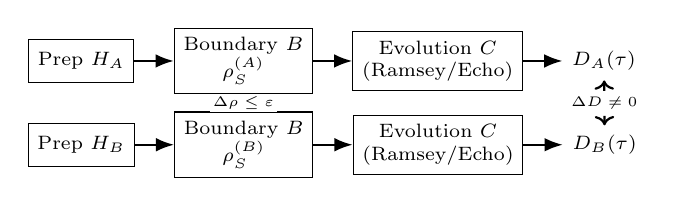
\begin{tikzpicture}[
    node distance=1.0cm and 0.4cm,
    box/.style={draw, rectangle, minimum height=0.55cm, font=\scriptsize, align=center},
    arrow/.style={-Latex, thick}
]
    % Top Row (History A)
    \node[box] (prepA) {Prep $H_A$};
    \node[box, right=0.5cm of prepA] (boundA) {Boundary $B$\\$\rho_S^{(A)}$};
    \node[box, right=0.5cm of boundA] (evolA) {Evolution $C$\\(Ramsey/Echo)};
    \node[right=0.5cm of evolA, font=\scriptsize] (resA) {$D_A(\tau)$};

    % Bottom Row (History B)
    \node[box, below=0.5cm of prepA] (prepB) {Prep $H_B$};
    \node[box, right=0.5cm of prepB] (boundB) {Boundary $B$\\$\rho_S^{(B)}$};
    \node[box, right=0.5cm of boundB] (evolB) {Evolution $C$\\(Ramsey/Echo)};
    \node[right=0.5cm of evolB, font=\scriptsize] (resB) {$D_B(\tau)$};

    % Arrows
    \draw[arrow] (prepA) -- (boundA);
    \draw[arrow] (boundA) -- (evolA);
    \draw[arrow] (evolA) -- (resA);

    \draw[arrow] (prepB) -- (boundB);
    \draw[arrow] (boundB) -- (evolB);
    \draw[arrow] (evolB) -- (resB);

    % Comparisons
    \draw[<->, dashed, thick] (boundA) -- node[fill=white, inner sep=1pt, font=\tiny] {$\Delta \rho \le \varepsilon$} (boundB);
    \draw[<->, dashed, thick] (resA) -- node[fill=white, inner sep=1pt, font=\tiny] {$\Delta D \neq 0$} (resB);
\end{tikzpicture}
\end{center}
\vspace{-0.5em}

\textbf{Null prediction (faithful state sufficiency).}
Assume that the reduced description at the conditioning boundary admits a \emph{faithful state representation} (Definition~\ref{def:faithful-state-representation}), such that admissible future evolution depends only on the boundary state and preserves admissible-history equivalence under all symmetry transformations that leave the reduced state invariant. Under this assumption, identical boundary states within the verified tolerance imply identical diagnostic behavior:
\[
D_A(\tau) = D_B(\tau) \quad \forall\, \tau .
\]

\textbf{Second-order prediction.}
If trajectory-level (second-order) constraints are physically relevant, then distinct admissible histories satisfying $\rho_B^{(A)} = \rho_B^{(B)}$ may nevertheless yield:
\[
D_A(\tau) \neq D_B(\tau).
\]

\textbf{Interpretation.}
A reproducible violation of the null prediction constitutes an operational failure of state sufficiency. Such a failure supports the presence of $\Sigma_2$-level constraint structure acting on admissible histories that is not representable within the reduced state alone. This result does not contradict the existence of global system--environment descriptions that restore Markovianity; it identifies the point at which such descriptions require representational enlargement beyond the reduced frame.

\end{tcolorbox}
\end{figure}

\paragraph{Null hypothesis (faithful state sufficiency).}
The null hypothesis tested by the protocol in Box~X assumes that the reduced
description at the conditioning boundary admits a \emph{faithful state
representation} in the sense of
Definition~\ref{def:faithful-state-representation}. Under this assumption,
admissible future evolution depends only on the boundary state and preserves
admissible-history equivalence under all symmetry transformations that leave the
reduced state invariant. Under faithful state sufficiency, identical verified
boundary states therefore imply identical diagnostic behavior for all subsequent
evolution.

\paragraph{Practical considerations.}
Implementing the protocol in Box~X requires careful control of boundary
verification and environmental coupling. Reduced-state tomography at the
conditioning boundary establishes operational indistinguishability at the level
of the verified description; it is not assumed to exhaust all global degrees of
freedom or correlations. The diagnostic tests whether such operationally
indistinguishable boundary states nevertheless admit distinct future extensions
under identical post-boundary evolution.

Persistent correlations established during the preparation histories
$H_A$ and $H_B$ constitute the signal of interest, as they encode admissible-history
structure beyond the reduced description. By contrast, deviations attributable
solely to active noise, experimental drift, or calibration error during the
post-boundary evolution must be excluded by independent controls.
\subsection{Falsification of the $\Sigma_2$ prediction}

The $\Sigma_2$ hypothesis makes a single falsifiable \emph{structural} claim:
within a fixed operational frame and under a boundary-symmetric reduction,
equality of reduced state at a conditioning boundary does not suffice to fix all
future reduced diagnostics when admissible history differs.

This claim is falsified if the following empirical condition holds.

\begin{quote}
\emph{For all admissible history pairs $H_A,H_B$ satisfying
$\rho_B^{(A)} = \rho_B^{(B)}$ under a boundary-symmetric operational reduction,
and for all subsequent evolution blocks $C$, the resulting reduced diagnostics are
statistically indistinguishable:
\[
D_A(\tau) = D_B(\tau)
\quad \text{for all probe parameters } \tau .
\]}
\end{quote}

Demonstrating this invariance across a sufficiently rich class of admissible
history constructions, conditioning procedures, and probe protocols would
establish that instantaneous reduced state suffices to characterize all
operationally accessible future behavior within the tested regime. In such a case,
no second-order constraint structure is required.

Conversely, the reproducible observation of history-dependent divergence
$D_A(\tau) \neq D_B(\tau)$ under verified boundary-state equality constitutes
direct evidence against state sufficiency. Under identical admissible dynamics and
post-boundary evolution, such divergence cannot be attributed to state-local
descriptions and therefore indicates irreducible trajectory dependence.

To distinguish genuine $\Sigma_2$ effects from finite-precision artifacts, the
protocol requires quantitative separation between diagnostic divergence and
boundary-state mismatch. Let $\varepsilon$ denote the verified upper bound on
state mismatch at the boundary (as determined by tomography or calibration), and
let $\Delta D(\tau) := |D_A(\tau) - D_B(\tau)|$. A $\Sigma_2$ signature is indicated
when
\[
\Delta D(\tau) \gg \mathcal{O}(\varepsilon)
\]
and persists under systematic refinement of boundary-state verification.

Operationally, this can be established by varying $\varepsilon$ through improved
control or post-selection while holding the admissible histories fixed. If
$\Delta D(\tau)$ extrapolates to a nonzero value as $\varepsilon \to$ its
experimental limit, the divergence cannot be attributed to incomplete state
matching.

The force of the test lies in its minimality. No modification of dynamics is
invoked, no ontological commitment to hidden variables is required, and no
environmental bookkeeping is assumed at the boundary. Any violation of the null
condition reflects a structural limitation of state-based descriptions within the
specified operational frame.

% --- Case studies ---
\section{Case Study: Measurement and Post-Selection}
\label{sec:case-measurement-postselection}

This section provides a concrete case study illustrating the necessity of
second-order constraint geometry $\Sigma_2$ within standard quantum-mechanical
practice.
The example concerns measurement and post-selection, chosen because it is
uncontroversial, operationally precise, and ubiquitous across quantum
experiments.

The analysis does not depend on interpretational commitments.
It relies only on standard measurement theory and experimentally realizable
protocols.

\subsection{Setup}

Consider a quantum system prepared in an initial state $\rho_0$ at time $t_0$.
At a later time $t_1$, a measurement is performed with outcomes labeled by
$i$, associated with measurement operators $\{M_i\}$ satisfying
$\sum_i M_i^\dagger M_i = \mathbb{I}$.

Upon obtaining outcome $i$, the system is assigned the post-measurement state
\[
\rho_i = \frac{M_i \rho_0 M_i^\dagger}{\mathrm{Tr}(M_i^\dagger M_i \rho_0)}.
\]

This update rule is standard and uncontroversial.

\subsection{State equivalence versus preparation equivalence}

Now consider an alternative preparation procedure in which the system is
directly prepared at time $t_1$ in the state $\rho_i$, without any prior
measurement or conditioning.

From the standpoint of quantum formalism, the two preparations are equivalent:
the system is described by the same density operator $\rho_i$, and all future
measurement statistics conditioned only on $\rho_i$ are identical.

However, the two preparations are not operationally equivalent in all contexts.

\subsection{Failure of admissibility equivalence}

Although the instantaneous states coincide, the admissibility of subsequent
operations may differ.

Examples include:
\begin{itemize}
\item extension of the system to a larger Hilbert space including an apparatus
      or environment,
\item reversal or partial reversal of the measurement interaction,
\item consistency of retrodictive inference about prior correlations.
\end{itemize}

In particular, a post-selected state $\rho_i$ obtained via measurement generally
does not admit a unitary extension that erases the measurement record without
access to additional degrees of freedom.
By contrast, a directly prepared state $\rho_i$ may admit such an extension.

This distinction cannot be recovered from the density operator alone.

\subsection{Second-order constraint interpretation}

From the standpoint of $\Sigma_2$, the difference between the two cases lies not
in the state but in the admissible histories leading to that state.

The post-selected ensemble is constrained by a conditioning boundary at the
measurement event.
Only trajectories consistent with outcome $i$ are admissible beyond that
boundary.

The directly prepared ensemble lacks this constraint.
Its admissible histories are not restricted by a prior measurement outcome.

Thus, the admissibility of future operations depends on ordered history, not
solely on instantaneous state.

The structural role of these measurement and post-selection examples can be made
explicit by relating them directly to the symmetry analysis in
Sec.~\ref{subsec:spin-half-symmetry-example}. In each case, admissible histories
that are operationally indistinguishable at the level of the reduced state
$\rho_S$ are related by transformations acting on degrees of freedom that are
inaccessible or uncontrolled from the perspective of the reduced description.
These transformations define an admissible-history symmetry: they act trivially
on instantaneous state but nontrivially on the space of histories by altering
which future operations (extensions, reversals, or conditional procedures)
remain physically realizable.

From this perspective, the distinction between directly prepared and
post-selected states is not merely a matter of system boundary specification.
Rather, it instantiates the same pattern identified in Sec.~3.5: a symmetry of
the admissible-history space arising from operational indistinguishability, whose
preservation prevents admissibility from factorizing through instantaneous state.
The failure of faithful state sufficiency here is therefore structural and
diagnostic, not an artifact of incomplete modeling or misuse of reduced states.

\subsection{Relation to irreversibility}

Having identified the symmetry-based origin of the admissibility distinction, this case study mirrors the structure identified in projection-induced arrow
analyses.
Measurement introduces a boundary-conditioned restriction on admissible
histories, even when subsequent dynamics are unitary.

Irreversibility arises not from intrinsic asymmetry in the dynamics, but from the
constraint imposed by conditioning.
This parallels the role of boundary selection in thermodynamic and decoherence
contexts.

\subsection{Why this is not an interpretational claim}

Nothing in this analysis asserts that quantum states are incomplete, hidden, or
epistemic.
The quantum formalism remains fully valid for predicting measurement statistics.

The point is classificatory:
state descriptions are sufficient for prediction, but not for admissibility.

$\Sigma_2$ provides a formal language for this distinction without modifying the
dynamics or adding variables.

\subsection{Summary}

Measurement and post-selection provide a minimal example in which:
\begin{enumerate}
\item identical quantum states arise from distinct preparation histories,
\item those histories impose different admissibility constraints,
\item the difference is not encoded in the instantaneous state.
\end{enumerate}

This establishes the necessity of second-order constraint structure in at least
one central domain of quantum practice.
\section{Case Study: Decoherence and Environmental Coupling}
\label{sec:case-decoherence-environment}

Decoherence provides a second canonical example in which instantaneous state
descriptions are insufficient to characterize admissible physical behavior.
Unlike measurement, decoherence involves no explicit projection postulate and
is often presented as fully reducible to unitary dynamics.
This makes it a particularly clean test case for the necessity of
second-order constraint structure.

\subsection{Standard decoherence setup}

Consider a system $S$ interacting unitarily with an environment $E$.
The joint state evolves according to
\[
\rho_{SE}(t) = U_{SE}(t)\,\rho_{SE}(0)\,U_{SE}^\dagger(t),
\]
with $U_{SE}$ generated by a time-reversal symmetric Hamiltonian.

Decoherence analyses typically focus on the reduced state
\[
\rho_S(t) = \mathrm{Tr}_E[\rho_{SE}(t)],
\]
whose off-diagonal terms in a preferred basis decay rapidly under generic
system–environment couplings.

\subsection{State-based description and its limits}

At any given time $t$, the reduced density matrix $\rho_S(t)$ provides a
complete description of all future measurement statistics on $S$ alone.
In this sense, decoherence introduces no deviation from standard quantum
mechanics.

However, the reduced state $\rho_S(t)$ does not encode the admissibility of
future operations that involve the environment.

In particular, two global histories can yield identical reduced states while
differing in whether recoherence, interference revival, or reversal operations
are physically realizable.

\subsection{History dependence of admissibility}

Consider two scenarios producing the same $\rho_S(t)$:

\begin{enumerate}
\item The system becomes entangled with a small, controllable environment,
      such that the joint evolution is, in principle, reversible.
\item The system becomes entangled with a large, uncontrolled environment,
      such that phase information is effectively dispersed into inaccessible
      degrees of freedom.
\end{enumerate}

At the level of $\rho_S(t)$, these scenarios are indistinguishable.
Yet the admissibility of subsequent operations—such as recoherence protocols,
Loschmidt echoes, or partial reversal—differs dramatically between them.

This distinction cannot be recovered from the instantaneous reduced state.

\subsection{Second-order constraint interpretation}

Within the $\Sigma_2$ framework, decoherence is understood as the imposition of
constraints on admissible histories rather than as a change in fundamental
dynamics.

Environmental coupling restricts the set of continuations compatible with a
given reduced state.
As entanglement spreads into uncontrolled degrees of freedom, the space of
admissible trajectories contracts.

Crucially, this contraction is path-dependent: it depends on how the system
arrived at its present reduced state, not merely on the state itself.

The decoherence and recoherence scenarios discussed in this section similarly
instantiate the symmetry-based diagnostic introduced in
Sec.~\ref{subsec:spin-half-symmetry-example}. Histories that yield the same reduced
state $\rho_S(t)$ may nonetheless differ in whether recoherence or reversal
operations are admissible, depending on correlations with environmental degrees
of freedom that are operationally inaccessible. Transformations acting on these
inaccessible degrees of freedom define an admissible-history symmetry: they leave
the reduced state invariant while acting nontrivially on the space of admissible
future continuations.

Viewed in this way, the insufficiency of the reduced state is not simply a
reminder that questions about joint system--environment operations require a
larger Hilbert space. Rather, it reflects the same structural situation identified
in Sec.~3.5: when admissibility depends on history-level relations preserved under
a physically motivated symmetry, no symmetry-preserving state representation can
encode all admissibility information. Decoherence thus provides a concrete
context in which second-order constraints arise as a representational issue,
independently of predictive success.

\subsection{Relation to arrow-like behavior}

Decoherence is often cited as explaining the emergence of classicality and
temporal asymmetry.
From the present perspective, this asymmetry arises from conditioning on
environmental correlations rather than from time-asymmetric laws.

This mirrors the structure identified in projection-induced arrow analyses:
the reduced description is anchored to a conditioning boundary that restricts
admissible histories in one direction.
The resulting arrow-like behavior is therefore boundary-relative, not intrinsic.

\subsection{Why decoherence does not eliminate $\Sigma_2$}

Decoherence is sometimes invoked as rendering higher-order structure unnecessary.
However, the symmetry-based diagnostic of Sec.~3.5 shows the opposite: decoherence makes second-order constraints unavoidable.

Even when all dynamics are unitary, the admissibility of operations depends on
ordered history, environmental accessibility, and prior entanglement structure.
These features are not representable within a purely state-based geometry.

\subsection{Summary}

Decoherence provides a paradigmatic case in which:
\begin{enumerate}
\item identical reduced states correspond to distinct admissible futures,
\item admissibility depends on environmental history and accessibility,
\item state descriptions suffice for prediction but not for operational reach.
\end{enumerate}

This establishes decoherence as a natural domain for second-order constraint
geometry and reinforces the general claim that $\Sigma_2$ captures structure
already implicit in quantum practice.
\section{Empirical Case Studies Relevant to $\Sigma_2$}
\label{sec:empirical-case-studies-sigma2}

This section surveys representative experimental classes in which observable
behavior is difficult to reconcile with state-sufficient descriptions, but arises
naturally once admissibility is treated as a property of histories rather than
instantaneous states. The goal is not to reinterpret quantum mechanics, but to
identify operational regimes in which state-based sufficiency fails.

Each case considered here is empirically robust, widely accepted within standard
quantum mechanics, and diagnostically useful because it isolates ordering or
trajectory dependence without introducing new dynamics or speculative mechanisms.

\subsection{Delayed-choice and retroactive conditioning experiments}

Delayed-choice experiments probe whether present measurement choices constrain
which histories are admissible, even when intermediate system descriptions are
identical across experimental branches. At the level of reduced state, the system
admits the same instantaneous description at the conditioning boundary, yet
subsequent choices alter the set of admissible continuations. Observable statistics
then diverge despite the absence of any state-local distinction at earlier times.

From a $\Sigma_2$ perspective, the diagnostic content of these experiments lies in
this mismatch between state equivalence and admissibility equivalence. The behavior
violates strict state sufficiency while remaining compatible with globally
constrained admissible histories, without invoking retrocausation or modified
dynamics.

\subsection{Postselection-induced statistical structure}

Postselected ensembles are common in quantum optics and weak measurement contexts.
Operationally, postselection generates ensembles whose statistics cannot be
reproduced by any convex mixture of forward-prepared states sharing the same
instantaneous description. This remains true even when disturbance and selection
bias are carefully controlled.

Within $\Sigma_2$, postselection is understood not as filtering states, but as
restricting admissible histories. The resulting statistical structure reflects
constraints on trajectory continuation rather than properties encoded in the
instantaneous system state. The failure of state sufficiency in this setting is
therefore operational and structural, not interpretive.

\subsection{Decoherence with history-dependent envelopes}

Standard decoherence theory assumes that reduced dynamics depend only on
instantaneous system--environment couplings. Empirically, however, decoherence
envelopes often depend on features of prior interaction history, including the
ordering and duration of earlier coupling regimes, even when reduced states and
instantaneous Hamiltonians are matched.

Such effects are commonly described as non-Markovian, presupposing an underlying
state description augmented by memory variables. $\Sigma_2$ offers a different
classification: admissible system--environment trajectories are globally
constrained, and this constraint persists even when no localized memory register
can be identified. The observed dependence therefore reflects a limitation of
state sufficiency rather than a failure of dynamical modeling.

\subsection{Interference recovery and which-path erasure}

Quantum eraser experiments demonstrate that interference can be recovered after
which-path information appears to have been irreversibly dispersed. In these
experiments, reduced system states can be operationally identical in cases with and
without recovered interference, while observable outcomes nevertheless differ.

From a second-order perspective, this distinction arises from admissible
correlation histories rather than from any restoration of instantaneous state
information. Interference recovery depends on trajectory-consistent erasure
conditions, not on state reconstruction. This directly exhibits failure of state
sufficiency without invoking hidden variables or retrocausal influence.

\subsection{Bell-type experiments and ordering dependence}

Bell inequality violations are often discussed in terms of nonlocal or contextual
state properties. However, Bell-type experiments also exhibit sensitivity to
measurement ordering, detector timing, and postselection criteria. These
sensitivities persist even when reduced states are operationally matched and cannot
be eliminated by state augmentation without introducing additional asymmetry.

$\Sigma_2$ reframes this behavior as arising from constraints on joint admissible
histories across spacelike-separated regions, rather than from violations of local
state realism. Importantly, this classification predicts no deviation from quantum
correlations. It predicts instead that attempts to restore state sufficiency via
hidden variables, retrocausal states, or enlarged ontologies encounter structural
obstructions tied to history-level admissibility.

\subsection{Macroscopic order-sensitive protocols}

Order dependence without state dependence is not confined to microscopic systems.
In controlled macroscopic protocols, identical initial and final states, identical
energy budgets, and identical instantaneous observables can nevertheless yield
distinct outcomes depending solely on the ordering of operations.

Such phenomena are often described as path dependence or hysteresis. Within
$\Sigma_2$, they are understood as macroscopic instances of the same structural
feature observed in microscopic settings: admissibility depends on trajectory even
when state-level descriptions agree. The distinction is therefore one of
representational regime, not of scale.

Across these diverse cases, a common diagnostic pattern emerges. Instantaneous
state descriptions fail to encode all operationally relevant constraints, while
history-level admissibility remains decisive. $\Sigma_2$ provides a unified
geometric language for this failure without introducing new dynamics or modifying
empirical predictions.

% --- Relations and implications ---
\section{Relation to Projection-Induced Arrows}
\label{sec:relation-projection-arrows}

The projection-induced arrow theorem and the second-order constraint geometry
$\Sigma_2$ address the same structural limitation from different descriptive
levels. The former establishes when arrow-like diagnostics are unavoidable under
operational reduction, while the latter identifies the minimal geometric structure
required once admissibility depends on history rather than instantaneous state.
This section makes their relationship explicit.

\subsection{Two views of the same limitation}

The projection-induced arrow result establishes a no-go constraint: under symmetric
admissible dynamics and boundary-symmetric operational reduction, no intrinsic
direction-sensitive diagnostic can arise. Any observed arrow must therefore enter
through asymmetry in dynamics, asymmetry in projection, or selection of a
conditioning boundary.

Second-order constraint geometry addresses the complementary question that follows
once this constraint is acknowledged. When admissibility depends on ordered
history rather than on instantaneous configuration, what structure is required to
represent that dependence without introducing spurious asymmetry?

In both frameworks, the answer is the same. Arrow-like behavior appears when future
realizability is constrained relative to a conditioning boundary in a manner that
cannot be represented at the level of instantaneous state.

\subsection{Projection as a special case of admissibility loss}

Operational projection $\Pi : \mathcal{H} \to \mathcal{D}$ discards relations among
histories that are relevant to admissibility. When the projection is
boundary-symmetric, this loss removes orientation information, forcing reduced
diagnostics to depend only on unsigned separation from the conditioning boundary.

This is a specific instance of a more general phenomenon. The reduced description
fails to encode which future histories remain admissible, not merely which states
are occupied. The loss is therefore operational rather than informational.

In the language of $\Sigma_2$, projection collapses distinct admissible-history
classes—each with different future-accessibility relations—into a single reduced
state. Arrow-like diagnostics then arise as a consequence of this collapse.

\subsection{Arrows as second-order constraints}

From the perspective of second-order constraint geometry, arrow-like diagnostics do
not measure intrinsic temporal direction. They quantify separation in admissibility
space from a conditioning boundary. Their magnitude reflects the accumulation of
constraints on which histories remain physically realizable.

This classification explains why arrow-like behavior is compatible with
time-reversal symmetric dynamics, insensitive to microscopic reversibility, and
dependent on preparation, conditioning, or environmental coupling. In each case,
the arrow reflects restrictions on admissible continuations rather than properties
of the equations governing evolution along a history.

\subsection{Boundary selection and admissibility}

The projection-induced arrow theorem deliberately remains agnostic about why a
particular conditioning boundary is physically realized. Second-order constraint
geometry sharpens this distinction by separating the role of boundary selection
from the structure of admissibility itself.

Boundary selection determines which admissibility constraints apply. $\Sigma_2$
determines how those constraints restrict future realizability once a boundary is
fixed. Maintaining this separation prevents a common category error: treating
boundary-relative directedness as evidence for intrinsic temporal asymmetry in the
dynamics.

\subsection{Unified structural interpretation}

Taken together, the two results yield a unified structural picture. Symmetric
admissible dynamics define the full space of possible histories. Operational
reductions identify histories that are distinct at the level of admissibility.
Boundary selection restricts which histories are physically realized. Second-order
constraint geometry encodes the resulting restrictions on future realizability,
and arrow-like diagnostics measure separation from the boundary within this
constrained admissibility structure.

In this sense, the projection-induced arrow theorem identifies the necessary
conditions under which arrows must appear, while $\Sigma_2$ provides the minimal
geometric language required to describe them once state sufficiency fails.

The recurrence of arrow-like phenomena across thermodynamics, decoherence, and
computation is therefore not a dynamical mystery. It is a structural consequence of
operating within reduced descriptions when admissibility depends on history rather
than on state.
\section{Relation to the Quantum Formalism}
\label{sec:comparison-quantum-formalism}

This section clarifies the relationship between second-order constraint geometry
$\Sigma_2$ and the standard quantum-mechanical formalism. The aim is neither to
revise nor to extend quantum mechanics, but to make explicit a structural feature
of its operational use: the reliance on admissibility constraints that are
history-dependent, even when expressed in state-based language.

Nothing in this section asserts a failure of quantum mechanics. The role of
$\Sigma_2$ is diagnostic and classificatory. It distinguishes structure that is
intrinsically state-local from admissibility relations that depend on ordered
history and are therefore not representable at the level of instantaneous state
alone.

\subsection{State sufficiency in the quantum postulates}

The quantum postulates assert that the physical state of a system at an instant of
time is fully specified by a state vector or density operator, and that future
measurement statistics are determined by this state together with the governing
Hamiltonian. Formally, this constitutes a first-order \emph{predictive} sufficiency claim: given $\rho(t)$, future statistics are fixed.

This claim is exact within the formal structure of the theory. However, the
operational deployment of quantum mechanics routinely invokes constraints that
are not encoded solely in the instantaneous state. These constraints become
visible when one asks not only what statistics will occur, but which operations,
extensions, or reversals are physically admissible.

\subsection{Preparation procedures and admissible histories}

Quantum predictions are conditioned on preparation procedures. Two density
operators may be mathematically identical while corresponding to preparation
histories that are not operationally interchangeable. Distinctions between
post-selected ensembles, decohered subsystems, and directly prepared states are
often suppressed once $\rho$ is specified, but reappear when considering which
future operations or embeddings remain admissible.

This indicates that admissibility is not exhausted by instantaneous state. The
quantum formalism remains predictively sufficient, but the admissible-history
structure on which those predictions rely is not fully represented at the state
level.

\subsection{Measurement update as a boundary-conditioned operation}

The measurement update rule introduces a non-unitary state change conditioned on a
specific outcome. This update is anchored at a definite boundary: the measurement
event. While the post-measurement state suffices for predicting subsequent outcome
statistics, the admissibility of the update itself presupposes an ordered history
that includes interaction, outcome registration, and conditioning.

From the perspective of $\Sigma_2$, this reflects an implicit boundary-conditioned
admissibility structure. Measurement theory operates successfully with this
structure in place, even though it is not represented explicitly as part of the
state description.

\subsection{Decoherence and environmental tracing}

Decoherence theory accounts for the suppression of interference by tracing over
environmental degrees of freedom. The resulting reduced density matrix often
appears diagonal in a preferred basis. However, the reduced state alone does not
encode whether coherence was lost through interaction or was never present. This
distinction is immaterial for many predictions, but becomes decisive when
considering reversibility, recoherence, or extension to a larger system.

The need to reference interaction history rather than instantaneous state is a
diagnostic signature of second-order constraint structure. It does not signal a
deficiency of the theory, but a limit of state-based representation.

\subsection{Unitary equivalence and admissible extension}

Quantum mechanics identifies states up to unitary equivalence. Unitary equivalence,
however, does not guarantee equivalence of admissible continuations. Reduced states
that are unitarily equivalent may differ in whether they admit consistent
reversal, extension to a larger Hilbert space, or recombination with previously
correlated subsystems.

Such distinctions do not contradict the formalism. They indicate that
admissibility relations are defined over histories and extensions, rather than
over instantaneous states alone.

\subsection{Structural clarification}

Second-order constraint geometry introduces no new variables, modifies no quantum
dynamics, and reinterprets no probabilities. It provides a language for
classifying when the successful use of quantum mechanics relies purely on state
sufficiency and when it relies on additional admissibility constraints introduced
by preparation, measurement, or reduction.

Recognizing these constraints explicitly sharpens the distinction between formal
predictive sufficiency and representational completeness. Quantum mechanics
remains correct and empirically validated; $\Sigma_2$ identifies the structural
regime in which state-based descriptions reach their natural limit.

\subsection{Relation to Consistent and Decoherent Histories}
\label{subsec:consistent-histories-relation}

The present framework bears a superficial resemblance to consistent and
decoherent histories (CH/DH) approaches, in that both treat histories rather than
instantaneous states as conceptually significant. It is therefore important to
clarify the precise relation and points of distinction.

Consistent histories formulations take histories as fundamental objects and
introduce consistency or decoherence conditions to ensure that probabilities can
be assigned to sets of histories without contradiction. These conditions restrict
which collections of histories may be treated as mutually exclusive and jointly
exhaustive alternatives. The primary aim is to extend probabilistic reasoning
beyond single-time measurements while retaining internal coherence of the
probability calculus.

Second-order constraint geometry addresses a different question. It does not
propose a new history-based formulation of quantum mechanics, nor does it impose
consistency conditions or define probability assignments over histories. Instead,
$\Sigma_2$ provides a diagnostic criterion for when state-based representations
fail to be faithful to admissible-history structure, independently of whether
probabilities over those histories are well defined.

A system may therefore satisfy the consistency criteria of the histories
framework while still failing to admit a faithful state-based representation of
admissibility in the sense of
Definition~\ref{def:faithful-state-representation}. In this sense, consistent
histories and $\Sigma_2$ are complementary but non-competing.

\subsection{Relation to Existing Literature}
\label{subsec:relation-existing-literature}

The perspective developed here intersects with several established frameworks in
quantum foundations, though its aims and conclusions are distinct. We briefly
situate second-order constraint geometry ($\Sigma_2$) relative to these approaches
to clarify both points of contact and departure.

\paragraph{Consistent and decoherent histories.}
The consistent histories program, introduced by Griffiths and further developed
by Omnès and others, treats histories as primary objects and imposes consistency
conditions to ensure that probabilities can be coherently assigned to sets of
histories \cite{griffiths1984consistent, griffiths2002consistent}. These
conditions restrict interference between histories so that classical probability
logic applies.

Second-order constraint geometry addresses a different question. It does not
impose consistency conditions, nor does it assign probabilities to histories.
Instead, $\Sigma_2$ diagnoses when admissibility of future operations fails to
factorize through instantaneous state, even when probabilities are well defined.

\paragraph{Decoherence and einselection.}
Decoherence theory, particularly as developed by Zurek, explains the emergence of
classical behavior via environmentally induced suppression of interference and
environment-induced superselection (einselection)
\cite{zurek1991decoherence, zurek2003decoherence}. These mechanisms operate
dynamically and statistically, identifying robust pointer states.

The present framework is orthogonal to these mechanisms. $\Sigma_2$ does not
address which states are dynamically selected, but whether admissibility of
operations can be represented faithfully at the level of instantaneous state.

\paragraph{Foundational no-go theorems.}
Results such as Bell’s theorem \cite{bell1964einstein} and the
Kochen--Specker theorem \cite{kochen1967problem} constrain state-based extensions
of quantum mechanics. Second-order constraint geometry does not propose such
extensions. It clarifies a different limitation: the failure of state-based
descriptions to encode admissibility relations under symmetry-preserving
representation, even when predictive completeness is preserved.

\paragraph{Trajectory-based and path-integral approaches.}
Trajectory-based and path-integral formulations emphasize histories as
computational tools. While they make essential use of trajectories, they do not
typically address when admissibility itself becomes history-dependent in a way
that cannot be compressed into state variables.

$\Sigma_2$ is agnostic to computational formalism. Its contribution is to identify
when history-level constraints are structurally irreducible under faithful,
symmetry-preserving state representation, regardless of the representational
technique employed.
\section{Why State Augmentation Does Not Restore Faithful Sufficiency}
\label{sec:why-state-augmentation-fails}

When empirical failures of state sufficiency are encountered, a standard response
is to enlarge the state description. Additional variables, hidden degrees of
freedom, memory registers, or extended ontologies are introduced with the aim of
restoring a first-order, state-based representation. The failure of state sufficiency discussed here is not a critique of standard open-system practice, but a classification of the representational regime in which such practice operates once reduced descriptions cease to be closed. In many cases, such
augmentations succeed in recovering predictive completeness.

The question addressed here is narrower and structural: whether such augmentations
can restore \emph{faithful} state sufficiency in the sense of
Definition~\ref{def:faithful-state-representation}. We argue that, when admissible
evolution depends irreducibly on ordered history, state augmentation may restore
prediction but cannot restore faithful representation. Trajectory dependence is
not eliminated; it is relocated.

Throughout this section, ``faithful'' is understood \emph{relative to a fixed
operational frame} (Sec.~\ref{sec:first-order-limits}): symmetries of the
admissible-history space are taken to represent experimentally verified
indistinguishabilities within that frame, and ``augmentation'' is counted as a
restoration of state sufficiency only when the added variables are independently
verifiable without leaving the frame.

\subsection{Predictive completeness versus representational faithfulness}

A state-based description is predictively complete if the augmented state suffices
to determine future statistics and admissible operations. Faithful sufficiency is
stronger: it requires that admissibility factor through state without breaking the
symmetry structure of the admissible-history space or introducing privileged
boundaries or orderings.

Once the ordering of prior transformations continues to constrain admissible
futures after the state is fixed, any augmentation that restores prediction must
encode that ordering explicitly or implicitly. The issue is therefore not whether
augmentation can succeed operationally, but whether it does so \emph{faithfully}.

\subsection{Hidden-variable extensions}

Hidden-variable theories illustrate the distinction clearly. If the additional
variables encode only instantaneous properties, ordering-sensitive admissibility
persists and sufficiency is not restored. If they encode sufficient historical
information to recover admissibility, the representation ceases to be faithful:
histories equivalent under the symmetries of $\mathcal{H}$ are mapped to distinct
augmented states.

In this case, predictive completeness is achieved only by breaking admissible-history
equivalence. The augmented state functions as a surrogate encoding of trajectory
classes rather than as a faithful instantaneous description.

\subsection{Memory variables and non-Markovian states}

A closely related strategy treats history dependence as a failure of Markovianity
and attempts to restore closure by introducing memory variables. While this move
often recovers predictive accuracy, it does so by explicitly embedding trajectory
information into the instantaneous description.

This is not a restoration of state sufficiency, but a relocation of the constraint.
The resulting object labeled as a ``state'' no longer represents a configuration
at an instant, but an equivalence class of histories summarized by a bookkeeping
variable. Calling such an object a state obscures the structural reality: admissibility
is determined by the path, not the point.

From the present perspective, non-Markovian state spaces are surrogate encodings of
trajectory-level constraints. They succeed computationally by forcing a history-based
process into a state-based form, but they do not eliminate second-order structure;
they conceal it.

Equivalently: when a ``memory kernel'' succeeds, it does so by importing
trajectory-level structure into an enlarged instantaneous description. $\Sigma_2$
does not deny the dynamical correctness of such models; it isolates when their
success depends on representational enlargement beyond the reduced frame.

\subsection{Extended Hilbert spaces and purification}

In quantum theory, mixed states are often purified by embedding the system into a
larger Hilbert space. At the global level, this restores unitary evolution. However,
it does not restore faithful state sufficiency at the operational level.

Reduced states remain insufficient to determine admissible continuations without
reference to preparation or selection history, and operational access to the
purifying degrees of freedom is typically restricted. As a result, purification
relocates admissibility constraints to an enlarged space without eliminating their
dependence on history or boundary conditions.

\subsection{Retrocausal and time-symmetric state assignments}

Retrocausal and time-symmetric formulations pursue predictive completeness by
allowing future boundary conditions to influence present state descriptions. While
such approaches may succeed operationally, they do so by abandoning local
state-based sufficiency altogether.

In terms of Definition~\ref{def:faithful-state-representation}, these formulations
encode admissibility constraints across entire histories rather than restoring a
faithful instantaneous representation. They are trajectory-based in substance,
even when expressed in state language.

\subsection{Why augmentation cannot be faithful in general}

All state-augmentation strategies share a common feature: they are justified solely by observed ordering dependence.
However, if admissibility depends on history relations invariant under the symmetries of $\mathcal{H}$ (i.e., relations preserved under experimentally verified indistinguishabilities), any state-based encoding that restores prediction effectively distinguishes between symmetry-equivalent histories. This conclusion holds for any finite or
countably infinite state augmentation,
provided the augmentation preserves the symmetry structure of the admissible-history
space rather than selecting privileged representatives.

This violates faithfulness. The augmentation succeeds operationally only by
introducing representational asymmetry, privileged boundaries, or explicit history
bookkeeping not present in the underlying admissible-history structure.

\subsection{Structural, not empirical, limitation}

The failure of faithful state augmentation is therefore structural rather than
empirical. It does not depend on experimental noise, incomplete control, or
approximation. Whenever admissibility depends irreducibly on ordered history, no state-based representation can be both predictively sufficient and faithful. This limitation is conditional rather than universal: it applies precisely in
regimes where admissibility relations are invariant under the symmetries of the
admissible-history space and cannot be factored through instantaneous state alone.

This result does not prohibit state augmentation, nor does it deny its practical
utility. It establishes a boundary: beyond a certain class of constraints,
augmentation restores prediction only by abandoning faithful representation.

\subsection{Relation to foundational no-go results}

This limitation parallels other foundational no-go statements. Just as no local
hidden-variable theory can faithfully reproduce quantum correlations, and no
noncontextual value assignment can faithfully represent measurement outcomes, so
no state-based augmentation can universally and faithfully restore sufficiency
across all admissible-history structures once admissibility depends on history.

Second-order constraint geometry makes this limitation explicit. It supplements
progressively more elaborate surrogate encodings with a minimal language in which
trajectory-dependent admissibility is represented directly rather than displaced.

Nothing in the present framework denies that state augmentation may succeed in restoring faithful sufficiency in many physical systems. In such cases, second-order constraint geometry adds no explanatory content and should not be invoked. The role of $\Sigma_2$ is strictly diagnostic: it becomes relevant only when predictive completeness is achieved at the cost of representational faithfulness.

\paragraph{Relation to non-Markovian descriptions.}
A standard response to history-dependent behavior is to embed the system into a
larger state space—typically by including environmental degrees of freedom—thereby
restoring Markovian evolution at the cost of state enlargement. Second-order
constraint geometry ($\Sigma_2$) does not deny the dynamical
correctness of this move, nor its predictive success. Instead, it diagnoses its representational cost.

Such embeddings succeed by relocating history dependence into an expanded instantaneous description. The crucial cost of this move is structural: the expanded description breaks the symmetries of the original operational frame.

By distinguishing between histories that are operationally indistinguishable at the conditioning boundary, the embedding introduces specific ordering or boundary information that is extrinsic to the reduced description. This diagnosis applies even when the added degrees of freedom are physically real. While ontologically valid in a global context, their inclusion alters the symmetry structure of the reduced theory by postulating distinctions that are not independently verifiable within the frame in which the reduced state is defined.

From the perspective of Definition~\ref{def:faithful-state-representation}, the result is therefore an unfaithful representation: predictive completeness is restored only by abandoning symmetry preservation. $\Sigma_2$ does not compete with non-Markovian models; it explains precisely when and why their success depends on symmetry-breaking augmentation rather than on genuinely state-local structure.
\section{Why Quantum Mechanics Is Not Wrong—but Structurally Limited}
\label{sec:qm-not-wrong-but-incomplete}

Quantum mechanics is among the most empirically successful frameworks in the
history of science. Its predictive accuracy, internal consistency, and
experimental confirmation are not in question. Nothing in the present work
challenges its formal structure, its dynamical laws, or its statistical
predictions.

The claim advanced here is narrower and structural. Quantum mechanics provides an
exact and complete account of states and their evolution, but it requires
supplementary operational structure in regimes where admissibility depends on
ordered history rather than instantaneous configuration alone. This requirement
does not reflect missing dynamics, incorrect equations, or empirical failure. It
reflects a representational limit of state-based description.

The quantum postulates assert that the physical state of a system at an instant of
time, together with the Hamiltonian, suffices to determine all future measurement
statistics. This first-order sufficiency claim is correct within the formalism and
adequate for a wide range of phenomena. However, it does not exhaust the question
of admissibility. In situations where future realizability depends on the
ordering of prior transformations, on preparation history, or on conditioning
procedures, the instantaneous quantum state remains predictive but does not
uniquely determine which future operations remain physically admissible.

In such cases, the quantum state is not incorrect. It is operationally
insufficient for encoding admissibility. Distinct histories may give rise to the
same reduced state while differing in which extensions, reversals, or control
operations remain realizable. This distinction is invisible at the level of
state description but decisive at the level of operational behavior.

Crucially, this limitation is not an interpretational issue. Competing
interpretations of quantum mechanics—collapse versus no collapse, epistemic
versus ontic states, many worlds versus hidden variables—agree on the same
predictions wherever state sufficiency holds. The phenomena motivating
$\Sigma_2$ arise when admissibility itself depends on history, even under fixed
state description. The issue therefore precedes any metaphysical interpretation
of the quantum state.

From this perspective, the persistent sense that quantum mechanics resists
intuition has a specific structural origin. The theory is extraordinarily precise
about states, amplitudes, and statistics, but largely silent about certain
ordering-dependent constraints that govern physical organization. These
constraints are operationally real and experimentally accessible, yet they are
not representable as properties of instantaneous states. Their absence from the
formalism reflects a boundary of representational scope, not a failure of the
theory.

This position does not conflict with existing no-go theorems. Results such as
Bell’s theorem, the Kochen--Specker theorem, and the no-cloning theorem restrict
state-based completions of quantum mechanics. Second-order constraint geometry
does not attempt such a completion. It introduces no hidden variables, modifies no
dynamics, and preserves all established impossibility results. Instead, it
clarifies when successful quantum descriptions rely on admissibility constraints
that are not encoded at the level of state alone.

Describing quantum mechanics as structurally limited in this sense is therefore
not a criticism. It is a statement about scope. Quantum mechanics is complete as a
theory of states and their evolution. It does not, in general, provide a complete
representation of admissible histories in regimes where ordering-sensitive
constraints matter. Recognizing this distinction explains why repeated attempts
to enforce universal state sufficiency encounter structural barriers rather than
empirical ones.

Second-order constraint geometry does not compete with quantum mechanics. It
articulates the boundary at which state-based description reaches its natural
limit and provides a minimal, non-dynamical language for expressing admissibility
structure that quantum theory already relies upon operationally but does not
itself encode.
\section{Implications for Quantum Measurement}
\label{sec:implications-quantum-measurement}

Quantum measurement is often regarded as the most persistent conceptual difficulty
in quantum theory because it appears to introduce a directional asymmetry that is
absent from the underlying dynamical laws. Measurements occur, outcomes are
recorded, and superpositions do not spontaneously reappear, even though unitary
quantum dynamics are time-reversal symmetric. This section clarifies the structural
origin of this asymmetry within the present framework.

The present work does not propose a collapse mechanism, modify unitary dynamics, or
introduce hidden variables. It addresses a narrower question: why measurement
exhibits arrow-like behavior even when the admissible dynamics themselves are
symmetric.

Within second-order constraint geometry, measurement is understood as the
imposition of a conditioning boundary. A measurement interaction and outcome
registration restrict which future histories remain admissible, independently of
the form of the underlying dynamics. This restriction is not representable as a
property of the instantaneous post-measurement quantum state. Once the boundary is
imposed, admissibility depends on the ordered sequence of events rather than on the
state alone.

From this perspective, the apparent irreversibility of measurement does not arise
from a dynamical prohibition against reversal. It arises because, after a
measurement boundary has been imposed, histories in which the outcome is undone are
no longer admissible under the operational constraints. Their exclusion follows
from admissibility structure rather than from any intrinsic time asymmetry in the
laws of motion.

This classification explains why measurement irreversibility is robust across
interpretations. Whether one adopts collapse models, many-worlds, or decoherence,
the operational asymmetry persists because it reflects a loss of state sufficiency
once history-dependent constraints are imposed. The asymmetry is therefore not an
interpretive artifact but a structural feature of admissible histories.

Decoherence fits naturally into this picture. Decoherence suppresses interference
between branches by projecting onto a reduced description relative to an
environmental partition. It does not, by itself, select a unique outcome. The
arrow-like behavior associated with decoherence arises when this projection is
combined with boundary selection that restricts admissible continuations. In this
sense, decoherence explains why certain superpositions become operationally
inaccessible, while second-order constraint geometry explains why accessibility
itself becomes history-dependent.

Measurement records are best understood not as stored states but as constraints on
future admissibility. Once a record exists, future operations must be consistent
with it. This is why arrow-like behavior appears even in minimal measurement-like
interactions, such as single-photon detection, post-selection, or weak measurement.
The macroscopic character of records is incidental; what matters is the imposition
of a second-order constraint on admissible histories.

Objective collapse models introduce explicit time-asymmetric dynamics in order to
account for measurement irreversibility. Within the present taxonomy, such models
address the problem by modifying the dynamics themselves. The approach developed
here neither endorses nor refutes these models. It clarifies that measurement
asymmetry can be understood without invoking intrinsic dynamical asymmetry, by
recognizing that measurement alters admissibility rather than state alone.

The contribution of the $\Sigma_2$ framework is therefore not a solution to the
measurement problem in the strong sense. It explains why the problem takes the form
it does. Measurement appears asymmetric because it changes the space of admissible
futures, and once this change occurs, no state-based description can fully encode
what has been excluded.
\section{Implications for Foundations and No-Go Theorems}
\label{sec:implications-no-go}

Modern foundations of physics are marked by a proliferation of no-go theorems:
results that prohibit entire classes of explanations rather than supplying
constructive alternatives. Bell nonlocality, Kochen--Specker contextuality,
no-cloning, no-broadcasting, and related results are typically treated as
independent constraints arising from distinct physical principles.

This section argues that many such results share a common structural source. They
arise when admissibility becomes history-dependent while the theory continues to
be represented in a state-sufficient language. The present framework does not
replace existing no-go theorems, but clarifies why they recur and why attempts to
evade them by state-based augmentation repeatedly fail.

Most foundational no-go results rely implicitly on the assumption that all
physically relevant constraints are encoded in an instantaneous state. This
assumption is rarely stated explicitly, but it underwrites demands such as
context-independent value assignment, factorization of joint probabilities,
local determination of outcomes, and the independence of future behavior from
preparation history once the state is fixed. Second-order constraint geometry
identifies this assumption as state sufficiency.

From this perspective, Bell’s theorem does not merely exclude local hidden
variables. It reveals that correlations observed in entangled systems cannot be
generated by descriptions that treat admissibility as state-local. The violation
of Bell inequalities indicates that admissible joint histories cannot be
decomposed into independent state assignments, even when those states are
operationally well defined. The failure lies not in locality alone, but in the
assumption that joint outcomes can be determined from local states without
reference to shared history.

A similar structural diagnosis applies to contextuality. The Kochen--Specker
theorem shows that context-independent value assignment is impossible. Within the
present framework, this follows directly from the fact that admissibility depends
on the ordering and compatibility of measurements. Different measurement contexts
impose different constraints on admissible histories, even when they act on the
same underlying system. Once admissibility is trajectory-dependent, contextuality
is not anomalous; it is unavoidable.

The same logic extends to no-cloning and no-broadcasting results. Cloning an
arbitrary quantum state would require that a single admissible history branch
into multiple future histories that preserve identical phase relations under all
possible subsequent operations. Such duplication is prohibited because
admissibility is not closed under unrestricted branching. From the standpoint of
$\Sigma_2$, no-cloning reflects a constraint on admissible trajectory structure,
not merely an algebraic feature of Hilbert space.

The recurrence of impossibility results across disparate formalisms and
interpretive programs is therefore not accidental. It signals a persistent
mismatch between representational assumptions and physical structure. As long as
theories are forced to encode history-dependent admissibility using
instantaneous state descriptions, contradictions and no-go results will continue
to emerge. These theorems are not failures of particular models, but diagnostics
of a deeper structural limitation.

This diagnosis parallels the projection-induced arrow result developed in the
companion paper. There, arrow-like directedness arises when state sufficiency
fails under conditioning, even though the underlying dynamics are symmetric.
Here, foundational no-go theorems arise when state sufficiency fails under
contextual and historical constraints. Both results instantiate the same
principle: state-based representations reach their limits whenever admissibility
depends on history rather than on instantaneous configuration.

The framework advanced here does not assert that quantum mechanics is
inconsistent, defective, or empirically incomplete. Quantum theory remains
extraordinarily successful as an operational and predictive framework. The claim
is structural rather than critical. Quantum mechanics encodes second-order
constraints using first-order representational tools, and no-go theorems mark the
boundaries of that encoding.

By locating these results within a unified constraint geometry, second-order
constraint theory clarifies why adding hidden variables, modifying dynamics, or
altering ontologies so often relocates foundational problems rather than resolves
them. The payoff is not a new ontology, but a clearer map of which explanatory
moves are structurally possible once admissibility is recognized as a property of
histories rather than states.

% --- Closing ---
\section{Conclusion}
\label{sec:conclusion}

This paper has shown that state sufficiency is not a universal representational
regime. There exist admissible dynamics for which future behavior depends on
ordering and trajectory constraints that cannot be recovered from instantaneous
state descriptions alone. When such dependence is present, a state-based geometry
is structurally incomplete as a faithful representation..

Within the state-sufficient regime, standard quantum mechanics remains correct and
operationally complete. Outside that regime, no modification of dynamics is
required. What is required is an additional geometric layer capable of expressing
constraints that act on admissible histories rather than on instantaneous states.
Second-order constraint geometry, $\Sigma_2$, provides this minimal structure.

The empirical content of the framework lies in the separation it enforces. By
holding reduced state statistics fixed while varying admissible history, the
protocols introduced here establish a sharp, falsifiable boundary between regimes
in which state sufficiency holds and regimes in which it fails. In the latter
case, history dependence is not an interpretive choice but an operational fact.

Together with the companion result on projection-induced arrows—which explains directional asymmetries under symmetric dynamics—this work clarifies exactly when and why state-based descriptions reach their limits. Arrows of directedness arise from projection; failures of state sufficiency arise from trajectory-level constraint structure. Both follow inevitably once admissible histories are taken as primary.

Second-order constraint geometry is therefore not an alternative theory, but the
next necessary layer of description when admissibility depends on history rather
than on state. Open questions include characterizing the full class of physically realizable $\Sigma_2$ structures, developing computational methods for identifying second-order constraints in complex systems, and exploring whether $\Sigma_2$ admits natural generalizations to higher-order trajectory dependence. The contribution is classificatory rather than predictive: it identifies when new predictions are impossible without expanding the representational frame.

\appendix
\section{Comparison with Related Frameworks}
\label{app:comparison-frameworks}

This appendix situates second-order constraint geometry ($\Sigma_2$) relative to existing formalisms in quantum foundations and open-system theory. The intent is not to claim priority or replacement, but to clarify the \emph{distinct role} played by $\Sigma_2$ as a diagnostic and classificatory layer.

Many established frameworks successfully model dynamics, probabilities, or causal structure. $\Sigma_2$ addresses a different question: \emph{when does a reduced, state-based description fail to faithfully represent admissibility without symmetry-breaking augmentation?}

Table~\ref{tab:comparison-frameworks} summarizes these relationships.

\begin{table}[htbp]
    \centering
    \small % Slightly reduces font size for better fit
    \renewcommand{\arraystretch}{1.4} % Adds breathing room between rows
    \caption{Comparison of $\Sigma_2$ with Related Frameworks}
    \label{tab:comparison-frameworks}
    
    % X columns automatically calculate width. 
    % >{\raggedright\arraybackslash} ensures text is left-aligned (not justified).
    \begin{tabularx}{\textwidth}{@{} >{\raggedright\arraybackslash}p{2.8cm} >{\raggedright\arraybackslash}X >{\raggedright\arraybackslash}X >{\raggedright\arraybackslash}X @{}} 
    \toprule
    \textbf{Framework} &
    \textbf{Primary Object} &
    \textbf{Sufficiency Criterion} &
    \textbf{Relation to $\Sigma_2$} \\
    \midrule
    
    Standard Quantum Mechanics &
    Instantaneous state $\rho(t)$ &
    \emph{Predictive} sufficiency: $\rho(t)$ fixes future statistics &
    $\Sigma_2$ does not challenge dynamical correctness; it diagnoses when predictive sufficiency fails to imply \emph{admissibility} sufficiency. \\
    
    Non-Markovian Dynamics &
    Augmented state or memory kernel &
    Restored Markovian closure via state enlargement &
    $\Sigma_2$ classifies when such augmentation restores prediction only by breaking admissible-history symmetries. \\
    
    Consistent Histories &
    Sets of histories $\{h\}$ with decoherence functional &
    Consistency of probability assignments over histories &
    Complementary: CH addresses probabilistic consistency; $\Sigma_2$ addresses representational sufficiency of reduced descriptions. \\
    
    Path Integral Formulation &
    Sum over trajectories &
    Global amplitude assignment &
    $\Sigma_2$ constrains admissibility of trajectories rather than computing amplitudes. No conflict with path-integral methods. \\
    
    Process Matrices / Quantum Combs &
    Higher-order maps on operations &
    Causal or operational consistency &
    $\Sigma_2$ is agnostic to causal ordering; it diagnoses failures of state-based sufficiency independently of causal structure. \\
    
    Causal Sets &
    Primitive causal relations &
    Causal consistency &
    Orthogonal: $\Sigma_2$ does not posit causal structure as fundamental, but constrains admissibility given fixed dynamics. \\
    
    Thermal Time Hypothesis &
    State-dependent notion of time &
    Thermodynamic consistency &
    Compatible: $\Sigma_2$ constrains admissible histories prior to time parametrization. \\
    \midrule
    
    \textbf{$\Sigma_2$ (This Work)} &
    \textbf{Admissible histories $\mathcal{H}$} &
    \textbf{\emph{Faithful} sufficiency:} factors through state without symmetry breaking &
    \textbf{Diagnostic and classificatory layer identifying structural limits of state-based descriptions.} \\
    
    \bottomrule
    \end{tabularx}
\end{table}

\paragraph{Interpretive neutrality.}
The classifications in Table~\ref{tab:comparison-frameworks} are intentionally interpretation-agnostic. Whether one adopts Everettian, consistent-histories, operational, or pragmatic open-systems viewpoints, the $\Sigma_2$ diagnostic applies whenever a reduced description is employed and admissibility depends on trajectory structure not factorizable through instantaneous state.

\paragraph{Scope.}
Nothing in this comparison asserts that $\Sigma_2$ is universally required. Closed systems, Markovian open systems, and many coarse-grained models remain faithfully state-sufficient. $\Sigma_2$ becomes relevant precisely when predictive completeness is achieved only by representational augmentation that breaks verified admissible-history symmetries.

\section{Derivation Details for the Concrete Hamiltonian Example}
\label{app:hamiltonian-derivation}

This appendix provides the explicit density-matrix and partial-trace derivations
supporting Sec.~\ref{subsec:concrete-hamiltonian-example}.
We show (i) equality of reduced boundary state under two admissible histories
within the reduced operational frame, and (ii) divergence of a reduced diagnostic
under identical post-boundary evolution.

\subsection{Setup and notation}

Let $S$ and $E$ be qubits with computational basis $\{\ket{0},\ket{1}\}$.
Define $\ket{+} := (\ket{0}+\ket{1})/\sqrt{2}$.
Let
\begin{equation}
H_{SE}=\hbar g\,\sigma_z^{(S)}\otimes \sigma_z^{(E)}, \qquad
U(t)=e^{-\frac{i}{\hbar}H_{SE}t}=e^{-i\phi\,\sigma_z^{(S)}\otimes\sigma_z^{(E)}},
\qquad \phi:=gt.
\end{equation}
On the joint computational basis $\ket{ij}\equiv \ket{i}_S\ket{j}_E$,
$\sigma_z^{(S)}\otimes\sigma_z^{(E)}$ has eigenvalue $+1$ on $\ket{00},\ket{11}$ and
$-1$ on $\ket{01},\ket{10}$, hence
\begin{equation}
U(\phi)\ket{00}=e^{-i\phi}\ket{00},\;
U(\phi)\ket{01}=e^{+i\phi}\ket{01},\;
U(\phi)\ket{10}=e^{+i\phi}\ket{10},\;
U(\phi)\ket{11}=e^{-i\phi}\ket{11}.
\label{eq:Uphi_action}
\end{equation}

We take the initial product state
\begin{equation}
\ket{\psi_0}=\ket{+}_S\otimes\ket{+}_E
=\tfrac{1}{2}\big(\ket{00}+\ket{01}+\ket{10}+\ket{11}\big).
\label{eq:psi0}
\end{equation}

Write the first interaction duration as $t_\theta$ with $\theta:=gt_\theta$,
and the post-boundary block duration as $t_\phi$ with $\phi:=gt_\phi$.

\subsection{Boundary states for the two histories}

\paragraph{History $H_A$.}
After the first interaction segment,
\begin{align}
\ket{\psi_A(B)} &= U(\theta)\ket{\psi_0}
\nonumber\\
&=\tfrac{1}{2}\Big(e^{-i\theta}\ket{00}+e^{+i\theta}\ket{01}+e^{+i\theta}\ket{10}+e^{-i\theta}\ket{11}\Big).
\label{eq:psiA_B}
\end{align}

\paragraph{History $H_B$.}
Apply $(\mathbb{I}_S\otimes\sigma_x^{(E)})$ after the first interaction segment:
since $\sigma_x\ket{0}=\ket{1}$ and $\sigma_x\ket{1}=\ket{0}$,
\begin{align}
\ket{\psi_B(B)} &=
(\mathbb{I}_S\otimes\sigma_x^{(E)})\,\ket{\psi_A(B)}
\nonumber\\
&=\tfrac{1}{2}\Big(e^{-i\theta}\ket{01}+e^{+i\theta}\ket{00}+e^{+i\theta}\ket{11}+e^{-i\theta}\ket{10}\Big)
\nonumber\\
&=\tfrac{1}{2}\Big(e^{+i\theta}\ket{00}+e^{-i\theta}\ket{01}+e^{-i\theta}\ket{10}+e^{+i\theta}\ket{11}\Big).
\label{eq:psiB_B}
\end{align}

\subsection{Reduced boundary density matrix $\rho_S(B)$}

Define $\rho_{SE}^{(A)}(B)=\ket{\psi_A(B)}\!\bra{\psi_A(B)}$ and
$\rho_{SE}^{(B)}(B)=\ket{\psi_B(B)}\!\bra{\psi_B(B)}$.
We compute $\rho_S^{(A)}(B)=\mathrm{Tr}_E[\rho_{SE}^{(A)}(B)]$ explicitly; the same
result holds for $H_B$ either by direct repetition or by the general invariance
$\mathrm{Tr}_E[(\mathbb{I}\otimes V)\rho(\mathbb{I}\otimes V^\dagger)]
=\mathrm{Tr}_E[\rho]$.

Write $\ket{\psi_A(B)}$ in Schmidt-like grouped form by environment basis:
\begin{equation}
\ket{\psi_A(B)}=
\ket{0}_E\otimes \ket{v_0}_S+\ket{1}_E\otimes \ket{v_1}_S,
\end{equation}
where (reading off coefficients from \eqref{eq:psiA_B})
\begin{equation}
\ket{v_0}_S=\tfrac{1}{2}\big(e^{-i\theta}\ket{0}+e^{+i\theta}\ket{1}\big),
\qquad
\ket{v_1}_S=\tfrac{1}{2}\big(e^{+i\theta}\ket{0}+e^{-i\theta}\ket{1}\big).
\label{eq:v0v1}
\end{equation}
Then
\begin{equation}
\rho_S^{(A)}(B)=\mathrm{Tr}_E\!\big[\ket{\psi_A(B)}\!\bra{\psi_A(B)}\big]
=\ket{v_0}\!\bra{v_0}+\ket{v_1}\!\bra{v_1}.
\label{eq:rhoS_sum}
\end{equation}
Compute each term using \eqref{eq:v0v1}:
\begin{align}
\ket{v_0}\!\bra{v_0}
&=\tfrac{1}{4}\Big(\ket{0}\!\bra{0}+\ket{1}\!\bra{1}
+e^{-i2\theta}\ket{0}\!\bra{1}+e^{+i2\theta}\ket{1}\!\bra{0}\Big),
\\
\ket{v_1}\!\bra{v_1}
&=\tfrac{1}{4}\Big(\ket{0}\!\bra{0}+\ket{1}\!\bra{1}
+e^{+i2\theta}\ket{0}\!\bra{1}+e^{-i2\theta}\ket{1}\!\bra{0}\Big).
\end{align}
Summing,
\begin{align}
\rho_S^{(A)}(B)
&=\tfrac{1}{2}\Big(\ket{0}\!\bra{0}+\ket{1}\!\bra{1}\Big)
+\tfrac{1}{4}\Big((e^{-i2\theta}+e^{+i2\theta})\ket{0}\!\bra{1}
+(e^{+i2\theta}+e^{-i2\theta})\ket{1}\!\bra{0}\Big)
\nonumber\\
&=\tfrac{1}{2}\mathbb{I}
+\tfrac{1}{2}\cos(2\theta)\Big(\ket{0}\!\bra{1}+\ket{1}\!\bra{0}\Big)
\nonumber\\
&=\tfrac{1}{2}\Big(\mathbb{I}+\cos(2\theta)\,\sigma_x^{(S)}\Big).
\label{eq:rhoS_B_final}
\end{align}
As noted, $\rho_S^{(B)}(B)=\rho_S^{(A)}(B)$ by the invariance of the partial trace
under local unitaries on $E$.

\subsection{Post-boundary evolution and reduced diagnostic}

Define the post-boundary evolution block as applying the \emph{same} unitary
$U(\phi)$ to both arms:
\begin{equation}
\ket{\psi_{A,2}}=U(\phi)\ket{\psi_A(B)}, \qquad
\ket{\psi_{B,2}}=U(\phi)\ket{\psi_B(B)}.
\end{equation}

\paragraph{Arm $A$.}
Using \eqref{eq:psiA_B} and the action \eqref{eq:Uphi_action},
\begin{align}
\ket{\psi_{A,2}}
&=\tfrac{1}{2}\Big(e^{-i(\theta+\phi)}\ket{00}+e^{+i(\theta+\phi)}\ket{01}
+e^{+i(\theta+\phi)}\ket{10}+e^{-i(\theta+\phi)}\ket{11}\Big)
\nonumber\\
&=U(\theta+\phi)\ket{\psi_0}.
\label{eq:psiA2}
\end{align}
Therefore, by repeating the boundary calculation with $\theta\mapsto(\theta+\phi)$,
the reduced state on $S$ satisfies
\begin{equation}
\rho_S^{(A)}(\phi)=\tfrac{1}{2}\Big(\mathbb{I}+\cos\big(2(\theta+\phi)\big)\sigma_x^{(S)}\Big),
\end{equation}
so the diagnostic $D(\phi):=\langle\sigma_x^{(S)}\rangle$ is
\begin{equation}
D_A(\phi)=\mathrm{Tr}\big(\rho_S^{(A)}(\phi)\sigma_x^{(S)}\big)=\cos\big(2(\theta+\phi)\big).
\label{eq:DA_final}
\end{equation}

\paragraph{Arm $B$.}
Start from \eqref{eq:psiB_B}, then apply $U(\phi)$:
\begin{align}
\ket{\psi_{B,2}}
&=\tfrac{1}{2}\Big(e^{-i\phi}e^{+i\theta}\ket{00}+e^{+i\phi}e^{-i\theta}\ket{01}
+e^{+i\phi}e^{-i\theta}\ket{10}+e^{-i\phi}e^{+i\theta}\ket{11}\Big)
\nonumber\\
&=\tfrac{1}{2}\Big(e^{-i(\phi-\theta)}\ket{00}+e^{+i(\phi-\theta)}\ket{01}
+e^{+i(\phi-\theta)}\ket{10}+e^{-i(\phi-\theta)}\ket{11}\Big)
\nonumber\\
&=U(\phi-\theta)\ket{\psi_0}.
\label{eq:psiB2}
\end{align}
Thus, again repeating the reduced-state calculation with angle $(\phi-\theta)$,
\begin{equation}
\rho_S^{(B)}(\phi)=\tfrac{1}{2}\Big(\mathbb{I}+\cos\big(2(\phi-\theta)\big)\sigma_x^{(S)}\Big),
\end{equation}
and
\begin{equation}
D_B(\phi)=\cos\big(2(\phi-\theta)\big).
\label{eq:DB_final}
\end{equation}

\paragraph{Divergence under identical boundary state.}
Equations \eqref{eq:rhoS_B_final}, \eqref{eq:DA_final}, and \eqref{eq:DB_final}
show:
\begin{itemize}
\item At the conditioning boundary $B$, $\rho_S^{(A)}(B)=\rho_S^{(B)}(B)$ exactly.
\item Under identical post-boundary evolution $U(\phi)$, the reduced diagnostics differ
for generic $(\theta,\phi)$:
\begin{equation}
D_A(\phi)=\cos\big(2(\theta+\phi)\big)\neq \cos\big(2(\phi-\theta)\big)=D_B(\phi).
\end{equation}
\end{itemize}
This is the explicit algebraic realization of the Box~X pattern:
operationally indistinguishable boundary states admit distinct future extensions.

\subsection{Partial-trace invariance under environment relabelings}

For completeness, we record the general identity used above.
For any operator $\rho_{SE}$ and any unitary $V_E$ on $E$,
\begin{equation}
\mathrm{Tr}_E\!\big[(\mathbb{I}_S\otimes V_E)\,\rho_{SE}\,(\mathbb{I}_S\otimes V_E^\dagger)\big]
=\mathrm{Tr}_E[\rho_{SE}],
\end{equation}
because the partial trace over $E$ is basis-independent and conjugation by a local
unitary on $E$ amounts to a change of basis on the traced subsystem.

\subsection{Symmetry group $G$ and operational indistinguishability}
\label{subsec:symmetry-group}

We now make explicit the symmetry structure underlying the concrete example
and show why any state augmentation that restores sufficiency necessarily
breaks a physically meaningful symmetry.

\paragraph{Operational frame.}
Fix the operational frame $F_S$ in which, at the conditioning boundary $B$,
only measurements and controls acting on the system $S$ are available.
No measurements on the environment $E$, joint $SE$ observables, or records
of intermediate operations are accessible in this frame.

Within $F_S$, two preparations are operationally indistinguishable at $B$
iff they induce identical reduced states $\rho_S(B)$ and yield identical
statistics for all observables accessible in $F_S$.

\paragraph{Definition of the symmetry group $G$.}
Let $G$ denote the group of transformations acting on admissible histories
that satisfy the following two conditions:
\begin{enumerate}
\item \textbf{State invariance:} For any $g\in G$ and any history $H$,
the induced reduced boundary state is invariant,
\[
\rho_S(B; H) = \rho_S(B; g\cdot H).
\]
\item \textbf{Operational undetectability:}
No measurement or control available in frame $F_S$ can detect whether $g$ has been applied.
That is, for any observable $O_S$ accessible in $F_S$ and any history $H$,
\[
\langle O_S \rangle_{H}
=
\langle O_S \rangle_{g \cdot H}.
\]
\end{enumerate}

In the present example, $G$ consists of all local unitaries acting on $E$
at the boundary,
\[
G = \{\, \mathbb{I}_S \otimes V_E \mid V_E \in \mathrm{U}(2) \,\}.
\]
Each $g\in G$ acts nontrivially on admissible histories but trivially on
the reduced boundary description in $F_S$.

\paragraph{Relation between the histories $H_A$ and $H_B$.}
The two histories introduced in
Sec.~\ref{subsec:concrete-hamiltonian-example} are related by the action
of a specific element of $G$:
\begin{equation}
H_B = (\mathbb{I}_S \otimes \sigma_x^{(E)}) \circ H_A .
\end{equation}
Explicitly,
\begin{equation}
\ket{\psi_B(B)} =
(\mathbb{I}_S \otimes \sigma_x^{(E)}) \ket{\psi_A(B)},
\end{equation}
as shown in Eq.~\eqref{eq:psiB_B}.
By invariance of the partial trace,
\begin{equation}
\rho_S^{(B)}(B)
=
\mathrm{Tr}_E\!\left[
(\mathbb{I}_S \otimes \sigma_x^{(E)})
\rho_{SE}^{(A)}(B)
(\mathbb{I}_S \otimes \sigma_x^{(E)})^\dagger
\right]
=
\rho_S^{(A)}(B),
\end{equation}
establishing that $H_A$ and $H_B$ are $G$-equivalent and
indistinguishable at the boundary within $F_S$.

\paragraph{Operational indistinguishability at the boundary.}
Let $O_S$ be any observable acting on $S$ accessible in $F_S$.
Then
\begin{equation}
\langle O_S \rangle_A
=
\mathrm{Tr}\!\left[\rho_S^{(A)}(B)\,O_S\right]
=
\mathrm{Tr}\!\left[\rho_S^{(B)}(B)\,O_S\right]
=
\langle O_S \rangle_B .
\end{equation}
Thus \emph{no measurement available in frame $F_S$ can distinguish}
$H_A$ from $H_B$ at the conditioning boundary.
The symmetry $G$ therefore corresponds to experimentally verified
indistinguishability, not merely formal equivalence.

\paragraph{Failure of faithful state augmentation.}
Suppose one attempts to restore state sufficiency by augmenting the reduced
state with an auxiliary variable $\lambda$ indicating which history occurred,
\[
\rho_S(B) \longmapsto (\rho_S(B), \lambda),
\qquad \lambda \in \{A,B\}.
\]
This augmentation distinguishes
\[
(\rho_S(B), A) \neq (\rho_S(B), B),
\]
despite the fact that:
\begin{enumerate}
\item $H_A$ and $H_B$ are related by a $G$-transformation,
\item all $G$-transformations are operationally undetectable in $F_S$,
\item no boundary-accessible measurement can determine $\lambda$.
\end{enumerate}

The augmented variable $\lambda$ therefore encodes distinctions that have
no operational support within the frame in which the reduced state is defined.
In the sense of Definition~\ref{def:faithful-state-representation},
this augmentation violates symmetry preservation and is unfaithful.

The divergence of diagnostics despite boundary-state equality
(Eqs.~\eqref{eq:diagnostic_divergence})
then follows as an operational consequence: future behavior depends on information
(the $G$-equivalence class of the history) that is not encoded in, and cannot be
recovered from, the reduced state $\rho_S(B)$ within frame $F_S$.

\paragraph{Physical meaning of symmetry breaking.}
To empirically verify the auxiliary variable $\lambda$ \emph{within frame $F_S$},
one would need to:
\begin{enumerate}
\item measure observables on $E$ (outside $F_S$ by definition),
\item perform joint $SE$ tomography (which requires access to $E$), or
\item retain records of the temporal ordering of operations during preparation
(requiring tracking of operations outside $F_S$).
\end{enumerate}

\textbf{Crucially, all of these operations are unavailable in frame $F_S$ by construction.}
Any measurement capable of verifying $\lambda$ would therefore constitute an
\emph{enlargement of the operational frame}, under which the $G$-equivalence
established at the boundary no longer holds.

Thus, postulating $\lambda$ as part of the state description within $F_S$ amounts
to claiming knowledge of information that is:
\begin{itemize}
\item not encoded in any $F_S$-accessible observable,
\item not verifiable by any measurement available at the boundary, and
\item only meaningful in an enlarged frame where $G$-symmetry is explicitly broken.
\end{itemize}

This is the precise sense in which state augmentation restores prediction only by
abandoning faithful representation: it imports distinctions from outside the
representational frame while claiming they belong inside it.

\paragraph{Analogy to gauge freedom.}
The situation is analogous to gauge freedom in electromagnetism:
different gauge choices yield identical physical predictions, yet any attempt to
promote gauge choice itself to a physical state variable breaks gauge invariance.
Here, $G$-equivalence classes play the role of gauge orbits, while the auxiliary
variable $\lambda$ functions as a gauge-fixing parameter that has no physical
meaning within the gauge-invariant (operationally reduced) description.

\paragraph{Optional frame refinement.}
If the operational frame is enlarged to $F_{SE}$, granting access to measurements
on $E$ at the boundary, the symmetry group contracts to the identity,
$G \to \{\mathbb{I}\}$, and state sufficiency is restored at the level of
$\rho_{SE}(B)$. The appearance of $\Sigma_2$ structure is therefore
frame-relative but non-arbitrary: it reflects objective operational
indistinguishability within the chosen frame.

\subsection{Remark on operational meaning}

In an operational frame $F_S$ where only $S$ is accessible at the boundary, the
two preparations are indistinguishable at $B$ because they induce identical
$\rho_S(B)$ and any boundary-accessible measurement is a function of $\rho_S(B)$.
Nevertheless, the fixed post-boundary interaction with $E$ makes the subsequent
reduced behavior depend on history-level information not recoverable from
$\rho_S(B)$ alone. This is precisely the representational regime that motivates
$\Sigma_2$ diagnostics.

\bibliographystyle{plain}
\bibliography{bib/references}

\end{document}